\documentclass[11pt]{article}
% new linux font, ignore mono
% \usepackage[mono=false]{libertine} 
% \renewcommand{\baselinestretch}{1.05}
% \usepackage[top=0.7in,left=1in,bottom=1in,right=1in]{geometry}
\usepackage{amsmath,amsthm,amssymb,epsfig,graphicx,mathrsfs,amsfonts,dsfont,bbm}
% \usepackage{bbm} % for \mathbb{1}, but ruins the letter
% \usepackage{unicode-math}
% \DeclareMathOperator*{\argmax}{argmax}
% \DeclareMathOperator*{\argmin}{argmin}
\usepackage{pict2e}
\usepackage[percent]{overpic}
\usepackage{color}
\usepackage{listings}
\usepackage{authblk}
\usepackage{caption}
% \usepackage{fullpage}
\usepackage[toc,title,titletoc,header]{appendix}
\usepackage{color}
\usepackage{dcolumn}
\usepackage{bm}
\usepackage{hyperref}
\hypersetup{
    citecolor=magenta,
    colorlinks=true,
    linkcolor=blue,
    filecolor=green,      
    urlcolor=cyan,
}
\usepackage[capitalise]{cleveref}
\usepackage{subcaption}
\usepackage{enumitem}
\usepackage{mathtools}
\usepackage{tikz}
% \usepackage{tikzit}
% \input{path_integral.tikzstyles}
% \usepackage{tkz-graph} % graph theory
\usepackage{braket}
\usepackage{physics}
% \usepackage{luatex85} % for qcircuit
\usepackage{luatex85,qcircuit}
\usepackage{blkarray}

% \setlength\parindent{0pt}
\setcounter{secnumdepth}{3}

\theoremstyle{plain}
\newtheorem{axiom}{Axiom}
\newtheorem{theorem}{Theorem}
\newtheorem{corollary}{Corollary}
\newtheorem{lemma}{Lemma}
\newtheorem{proposition}{Proposition}
\newtheorem{conjecture}{Conjecture} 
\newtheorem{question}{Question} 
\newtheorem{claim}{Claim} 
\theoremstyle{definition}
\newtheorem{definition}{Definition}
\newtheorem{observation}{Observation} 
\newtheorem{fact}{Fact}
\newtheorem{example}{Example}
\newtheorem{remark}{Remark}
\newtheorem{problem}{Problem}

\usepackage[margin=2cm]{geometry}

% bib title hyperlink
\usepackage[style=alphabetic,doi=false,url=false,isbn=false,backend=biber,backref=true]{biblatex}
% \DefineBibliographyStrings{english}{%
%   backrefpage = {p.},% originally "cited on page"
%   backrefpages = {pages},% originally "cited on pages"
% }
% \AtEveryBibitem{
%     \clearfield{urlyear}
%     \clearfield{urlmonth}
% }
% \addbibresource{bib.bib}
% \addbibresource{ref.bib}
\addbibresource{~/GitHub/Self-Study-Notes-on-Quantum-Computation/ref.bib}
% \addbibresource{Quantum_Computation.bib}
% \addbibresource{Quantum_Physics.bib}
% \addbibresource{Textbook.bib}
% \addbibresource{CS.bib}
% \addbibresource{Math.bib}

\newbibmacro{string+doiurlisbn}[1]{%
    \iffieldundef{doi}{%
    \iffieldundef{url}{%
        \iffieldundef{isbn}{%
        \iffieldundef{issn}{%
            #1%
        }{%
            \href{http://books.google.com/books?vid=ISSN\thefield{issn}}{#1}%
        }%
        }{%
        \href{http://books.google.com/books?vid=ISBN\thefield{isbn}}{#1}%
        }%
    }{%
        \href{\thefield{url}}{#1}%
    }%
    }{%
    \href{http://dx.doi.org/\thefield{doi}}{#1}%
    }%
}

\DeclareFieldFormat[article,incollection,inproceedings,book,misc,online]{title}{\usebibmacro{string+doiurlisbn}{#1}}
\DeclareFieldFormat{journaltitle}{\mkbibemph{#1}\isdot}
\DeclareFieldFormat{booktitle}{#1\isdot}
\renewbibmacro{in:}{}

% !TEX root = ./graph_kernel.tex

%%%%%%%%%%%%%%%%%%%%%%%%%%%%%%%%%%%%
%%%%%%%%%%%%%% math %%%%%%%%%%%%%%%%
%%%%%%%%%%%%%%%%%%%%%%%%%%%%%%%%%%%%
\newcommand{\calH}{\mathcal{calH}}
\newcommand{\hilbertspace}{\mathcal{H}}
\newcommand{\bigO}{\mathcal{O}}
\newcommand{\lagrangian}{\mathcal{L}}
\newcommand{\VS}{\textrm{VS}}

\newcommand{\realnumber}{\mathbb{R}}
\newcommand{\complexnumber}{\mathbb{C}}
\newcommand{\rationalnumber}{\mathbb{Q}}
\newcommand{\integer}{\mathbb{Z}}
\newcommand{\naturalnumber}{\mathbb{N}}
\newcommand{\numberfield}{\mathbb{F}}

\newcommand{\0}{\mathbf{0}}
\newcommand{\bI}{\mathbf{I}}
\newcommand{\identity}{\mathds{1}}
\newcommand{\midentity}{\mathds{1}}
% \newcommand{\identity}{\mathbb{1}}
\newcommand{\bX}{\mathbf{X}}
\newcommand{\bY}{\mathbf{Y}}
\newcommand{\bepsilon}{\boldsymbol{\epsilon}}

\newcommand{\ii}{\textup{i}}

\newcommand{\floor}[1]{\left\lfloor #1 \right\rfloor}
\newcommand{\ceil}[1]{\left\lceil #1 \right\rceil}

% probability
\newcommand{\probability}{\mathbb{P}}
\newcommand{\variance}{\textup{\textrm{Var}}}
\newcommand{\covariance}{\textup{\textrm{Cov}}}
\newcommand{\expectation}{\mathbb{E}}

% group theory
\newcommand{\group}{\mathbb{G}}
\newcommand{\dihedral}{\mathbb{D}}
\newcommand{\GL}{\mathbb{GL}}
\newcommand{\SL}{\mathbb{SL}}
\newcommand{\Sp}{\textup{Sp}}
% \newcommand{\sp}{\mathfrak{sp}}
\newcommand{\SU}[1]{\textup{SU(#1)}}
\newcommand{\su}[1]{\mathfrak{su}(#1)}
% \renewcommand{\SO}[1]{\textup{SO(#1)}}
% \newcommand{\SO}{\textup{SO}}

% graph theory
\newcommand{\graph}{G}

% matrix and linear algebra
\newcommand{\diag}{\textup{diag}}
% \let\span\relax
% \DeclareMathOperator{\span}{\textup{span}}
% \newcommand{\span}{\textup{span}}
\newcommand{\spn}{\mathop{\mathrm{span}}}
\DeclareMathOperator{\spann}{\textup{span}}
%%%%%%%%%%%%%%%%%%%%%%%%%%%%%%%%%%%%
%%%%%%%%%%%%%%  CS  %%%%%%%%%%%%%%%%
%%%%%%%%%%%%%%%%%%%%%%%%%%%%%%%%%%%%
% cryptography
\newcommand{\gen}{\textsf{Gen}}
\newcommand{\enc}{\textsf{Enc}}
\newcommand{\dec}{\textsf{Dec}}
\newcommand{\mac}{\textsf{Mac}}
\newcommand{\sign}{\textsf{Sign}}
\newcommand{\verfy}{\textsf{Verfy}}
\newcommand{\negl}{\textup{negl}}

% quantum computing
% gates
\newcommand{\cnot}{\textup{\textsc{cnot}}}
\newcommand{\hdm}{\textup{\textsc{h}}}
\newcommand{\tphase}{\textup{\textsc{t}}}
\newcommand{\cphase}{\textup{\textsc{cphase}}}
\newcommand{\swap}{\textup{\textsc{swap}}}
\newcommand{\negate}{\textup{\textsc{not}}}
\newcommand{\QFT}{\textup{QFT}}

% Boolean Functions
\newcommand{\MAJ}{\textup{\textsc{maj}}}
\newcommand{\NOT}{\textup{\textsc{not}}}
\newcommand{\OR}{\textup{\textsc{or}}}
\newcommand{\AND}{\textup{\textsc{and}}}
\newcommand{\NAND}{\textup{\textsc{nand}}}
\newcommand{\EQ}{\textup{\textsc{eq}}}
\newcommand{\IP}{\textup{\textsc{ip}}}
\newcommand{\DISJ}{\textup{\textsc{disj}}}
\newcommand{\Parity}{\textup{\textsc{parity}}}
\newcommand{\Threshold}{\textup{\textsc{thr}}}

\newcommand{\GS}{\textup{\textsc{gs}}}
\newcommand{\dejo}{\textup{\textsc{DeJo}}}
\newcommand{\STAB}{\textup{\textsc{stab}}}

% algorithms
\newcommand{\algo}{\mathcal{A}}
\newcommand{\maxcut}{\textup{\textsc{MaxCut}}}
\newcommand{\sat}{\textup{\textsc{sat}}}
\newcommand{\partition}{\textup{\textsc{Partition}}}
\newcommand{\bosonsample}{\textup{\textsc{BosonSampling}}}

% complexity measures
\newcommand{\vcdim}{\mathsf{VCdim}}
\DeclareMathOperator{\certificate}{\mathsf{Cert}}
\DeclareMathOperator{\s}{\mathsf{s}}
\DeclareMathOperator{\bs}{\mathsf{bs}}
\DeclareMathOperator{\adeg}{\mathsf{\widetilde{deg}}}
% \DeclareMathOperator{\adv}{\mathsf{Adv}}
\DeclareMathOperator{\dqc}{\mathsf{D}}
\DeclareMathOperator{\rqc}{\mathsf{R}}
\DeclareMathOperator{\qqc}{\mathsf{Q}}
\DeclareMathOperator{\cmc}{\mathsf{C}}
\DeclareMathOperator{\rcmc}{\mathsf{RC}}
\DeclareMathOperator{\qcmc}{\mathsf{QC}}
\let\deg\relax
\DeclareMathOperator{\deg}{\mathsf{deg}}
\DeclareMathOperator{\poly}{\textup{poly}}

% complexity classes
\newcommand{\reduceto}{\le_P}
\let\cclass\textup
\let\P\relax
\newcommand{\P}{\cclass{P}}
\newcommand{\PP}{\cclass{PP}}
\newcommand{\NP}{\cclass{NP}}
\newcommand{\sharpP}{\cclass{\#P}}
\newcommand{\coNP}{\cclass{co-NP}}
\newcommand{\PH}{\cclass{PH}}
\newcommand{\NPC}{\cclass{NPC}}
\newcommand{\BQP}{\cclass{BQP}}
\newcommand{\QMA}{\cclass{QMA}}
\newcommand{\PSPACE}{\cclass{PSPACE}}
\newcommand{\BPP}{\cclass{BPP}}

% Optimization
\newcommand{\subjectto}{\textup{subject to  }}

\let\iff\relax
\newcommand{\iff}{\text{ iff }}
\newcommand{\eff}{\textup{eff}}
\newcommand{\st}{\text{ s.t. }}
\newcommand{\otherwise}{\text{otherwise}}
\newcommand{\T}{\intercal}
\newcommand{\OPT}{\textup{OPT}}


\newcommand\vartextvisiblespace[1][.5em]{%
  \makebox[#1]{%
    \kern.07em
    \vrule height.3ex
    \hrulefill
    \vrule height.3ex
    \kern.07em
  }% <-- don't forget this one!
}
\newcommand{\visiblespace}{\vartextvisiblespace}

%%%%%%%%%%%%%%%%%%%%%%%%%%%%%%%%%%%%
%%%%%%%%%%%%% Physics %%%%%%%%%%%%%%
%%%%%%%%%%%%%%%%%%%%%%%%%%%%%%%%%%%%
\newcommand{\zpartition}{\mathcal{Z}}
\newcommand{\llaplacian}{\mathfrak{L}}
\newcommand{\dlagrangian}{\mathcal{L}}
\newcommand{\eaction}{\mathcal{S}_{\textup{E}}}
\newcommand{\action}{\mathcal{S}}
\newcommand{\hhat}{\hat{H}}
\newcommand{\xhat}{\hat{x}}
\newcommand{\phat}{\hat{p}}
\newcommand{\qhat}{\hat{q}}
\newcommand{\nhat}{\hat{n}}
\newcommand{\pihat}{\hat{\pi}}
\newcommand{\phihat}{\hat{\phi}}
\newcommand{\oph}{\mathbf{H}}
\newcommand{\opx}{\mathbf{x}}
\newcommand{\opp}{\mathbf{p}}
\newcommand{\opq}{\mathbf{q}}
\newcommand{\vecx}{\vec{x}}
\newcommand{\vecp}{\vec{p}}
\newcommand{\veck}{\vec{k}}
\newcommand{\vecq}{\vec{q}}
\newcommand{\vbk}{\vb{k}}
\newcommand{\vbx}{\vb{x}}
\newcommand{\vbn}{\vb{n}}
\newcommand{\vbp}{\vb{p}}
\newcommand{\vbq}{\vb{q}}
\newcommand{\vbr}{\vb{r}}
\newcommand{\vbe}{\vb{e}}
\newcommand{\vbv}{\vb{v}}
\newcommand{\vbw}{\vb{w}}
\newcommand{\vbB}{\vb{B}}
% \newcommand{\acreation}{\hat{a}^\dagger}
% \newcommand{\aannihilation}{\hat{a}}
\newcommand{\acreation}{\hat{a}^\dagger}
\newcommand{\aannihilation}{\hat{a}}
\newcommand{\bcreation}{\hat{b}^\dagger}
\newcommand{\bannihilation}{\hat{b}}
\newcommand{\ccreation}{\hat{c}^\dagger}
\newcommand{\cannihilation}{\hat{c}}
\newcommand{\homega}{\hbar \omega}
\newcommand{\opsigma}{\hat{\bm{\sigma}}}
\newcommand{\hatsigma}{\hat{\sigma}}
\newcommand{\bmhsig}{\bm{\hat{\sigma}}}
\newcommand{\hsig}{\hat{\sigma}}
\newcommand{\si}{\hat{\sigma}_0}
\newcommand{\sx}{\hat{\sigma}_x}
\newcommand{\sy}{\hat{\sigma}_y}
\newcommand{\sz}{\hat{\sigma}_z}
\newcommand{\splus}{\hat{\sigma}_+}
\newcommand{\sminus}{\hat{\sigma}_-}
\newcommand{\px}{\hat{X}}
\newcommand{\py}{\hat{Y}}
\newcommand{\pz}{\hat{Z}}
\newcommand{\pI}{\hat{I}}
\newcommand{\schrodinger}{\textup{Schr\"{o}dinger }}
\newcommand{\tc}{T_c}
\newcommand{\alembertian}{\square}
\newcommand{\vecA}{\vb{A}}
\newcommand{\magfield}{\vb{B}}
\newcommand{\elefield}{\vb{E}}

\newcommand{\deltat}{\Delta t}
\newcommand{\deltatau}{\Delta \tau}

%%%%%%%%%%%%%%%%%%%%%%%%%%%%%%%%%%%%
%%%%%%%%%%%%% Quantum Computing %%%%%%%%%%%%%%
%%%%%%%%%%%%%%%%%%%%%%%%%%%%%%%%%%%%
% \newcommand{\gcommutator}[1]{[[ #1 ]]}
\usepackage{stmaryrd}
\newcommand{\gcommutator}[1]{\llbracket #1 \rrbracket}
\newcommand{\subgroup}{\mathbb{H}}
\newcommand{\dlog}{\textsf{DLog}}
\newcommand{\hsp}{\textsf{HSP}}
\renewcommand{\llaplacian}{\hat{\mathfrak{L}}}
% \newcommand{\zpartition}{\mathcal{Z}}
\newcommand{\hamiltonian}{\hat{H}}
\newcommand{\U}{\hat{U}}
\newcommand{\inputspace}{\mathcal{X}}
\newcommand{\kernel}{\mathcal{K}}
\newcommand{\D}{\mathcal{D}}
\newcommand{\oracle}{\hat{O}}
\newcommand{\proj}{\hat{P}}
% \newcommand{\deltat}{\Delta t}
% \newcommand{\deltatau}{\Delta \tau}
\newcommand{\cz}{\textup{\textsc{cZ}}}
\newcommand{\cx}{\textup{\textsc{cx}}}
\newcommand{\toffoli}{\textup{\textsc{toffoli}}}
\newcommand{\lleft}{\leftarrow}
\newcommand{\rright}{\rightarrow}
\newcommand{\intinf}{\int_{-\infty}^{\infty}}


%%%%%%%%%%%%%%%%%%%
\title{Manuscript: Quantum Graph Kernels, Symmetries, and Speedups}
\author{Jue Xu\footnote{\href{mailto:juexu@cs.umd.edu}{ juexu@cs.umd.edu}} }
% \email{juexu@umd.edu}  
% \affil{University of Maryland, College Park}
%%%%%%%%%%%%%%%%%%%

\begin{document}
% \vspace{10mm}
\maketitle
\begin{abstract}
	We discuss the quantum analogues of kernel methods for quantum machine learning.
	% We discuss the quantum analogue of graph kernels based on quantum random walks. 
	Moreover, both theoretical and heuristic quantum advantages in machine learning are investigated, mainly in terms of structures (symmetries) of problems.
	% motivation
\end{abstract}

\setcounter{tocdepth}{2}
\tableofcontents
% \newpage

%%%%%%%%%%%%%%%Content%%%%%%%%%%%%%%%
% !TEX root = ./main.tex

\section{Introduction}
% \subsection{Motivation}
With the success of machine learning and potential advantages of quantum computing [ref], the combination of these two areas attracts attention.
Many quantum versions of machine learning techniques \cite{rebentrostQuantumSupportVector2014} \cite{lloydQuantumPrincipalComponent2014} \cite{congQuantumConvolutionalNeural2019} are developed and exhibtis substantial (meaningful) speedups.
However, the quantum advantages are heuristic and strongly depend on the assumptions of models \cite{tangQuantumPrincipalComponent2021}.
Since several quantum kernel tricks are coined \cite{havlicekSupervisedLearningQuantum2019} \cite{schuldQuantumMachineLearning2019} and advantages are demonstrated \cite{glickCovariantQuantumKernels2021} \cite{liuRigorousRobustQuantum2021},
we focus on quantum graphs kernel based on quantum random walk. 
The (rigorous) quantum advantages in this context are analyzed in terms of symmetries by theoretical group methods \cite{kondorGroupTheoreticalMethods2008} \cite{ben-davidSymmetriesGraphProperties2020}.
On the other hand, the (empirical) connections between quantum machine learing and quantum physics are revealed by symmetries.
% diffusion kernel on graphs \cite{kondorDiffusionKernelsGraphs2002}

% Many insightful and powerful models, like adiabatic quantum computation \cite{farhiQuantumComputationAdiabatic2000}, quantum random walks \cite{childsQuantumInformationProcessing2004} \cite{ambainisOnedimensionalQuantumWalks2001}, 

\subsection{Preliminary and Notation}
In this work, we restrict ourself to supervised learning (mainly SVM), where we are given a set of labeled data for training to predict labels of new data.
The (classical) training data is a set of $m$ data points $\qty{(\vbx^{(i)}, y^{(i)})}^{m}_{i=1}$ 
where each data point is a pair $(\vbx,y)$.
Normally, the input $\vbx:= (x_1,x_2,\dots,x_d) \in \realnumber^d$  is a vector where $d$ is the number of \emph{features}
and its \emph{label} $y\in\Sigma$ is a scalar with some discrete set $\Sigma$ of alphabet/categories. 
For simplicity, we assume $\Sigma=\qty{-1,1}$ (binary classification).

graph $\graph=(V,E)$, group $\group$. 
operator $\hat{A}$, $\hamiltonian$

computational basis $\ket{z}$ with $z\in \qty[2^n]$ where $n$ is the number of qubits,
the binary representation $\ket{\vbx}=\ket{x_1,x_2,\dots,x_n},x_j\in \qty{0,1}$. 
Let $N \equiv 2^n$ if no ambiguity.
$\ket{\vb{0}}\equiv\ket{0}^n$, $\ket{\pm}$.
% \subsubsection{Support Vector Machine (SVM)}
% \subsubsection{Kernel trick}
% \subsubsection*{Hilbert space}
inner product can be understood as a `similarity' metric between two vectors ?
\begin{definition}[inner product]\label{def:inner_product}
	An \emph{inner product} is a map
	$\expval{\cdot,\cdot}: \mathcal{V} \times \mathcal{V} \to \numberfield$
	where $\mathcal{V}$ is a vector space and $\numberfield$ is...
	% \begin{equation}
	% 	\expval{\cdot,\cdot}: V \times V \to \numberfield
	% \end{equation}
	And $\forall \vbx,\vb{y},\vb{z}\in V,a,b\in\numberfield$, 
	the map satisfies the following three properties:
	\begin{itemize}
		\item \textbf{Conjugate symmetry}:
		$\expval{\vbx,\vb{y}}=\overline{\expval{\vb{y},\vbx}}$
		\item \textbf{(Bi)Linearity}:
		$\expval{a\vbx+b\vb{y},\vb{z}}=a\expval{\vbx,\vb{z}}+b\expval{\vb{y},\vb{z}}$
		\item \textbf{Positive-definiteness}:
		$\expval{\vbx,\vbx}\ge 0$ with equality only when $\vbx=\vb{0}$.
	\end{itemize}
	In classical machine learning, we assume the base field is $\realnumber$.
	The inner product gives rise to the \emph{norm} $\norm{\vbx}=\sqrt{\expval{\vbx,\vbx}}$,
	and a distance metric $d(\vbx,\vbx')=\norm{\vbx-\vbx'}$.
	dot product
\end{definition}
Euclidean vector space $\realnumber^n$ with dot product is an inner product space,.
While in the context of quantum mechanics,
the inner product is replaced by 
Dirac notation $\braket{\vbx}{\vbx'}$ with complex field $\complexnumber$.
\begin{definition}[Hilbert space]\label{def:hilbert_space}
	A \emph{Hilbert space} is a vector space $\hilbertspace$ induced by an \nameref{def:inner_product}
	such that the inner product yields a complete metric space?.
\end{definition}

\subsection{Background: SVM and kernel trick}\label{sec:svm}
\emph{Support vector machine} (SVM) is one of popular \emph{supervised learning} techniques \cite{cortesSupportvectorNetworks1995}.
% \footnote{unsupervised learning}
% \subsubsection{Support Vector Machine (SVM)}
training stage, classification stage (phase).
exponentially large space;
($n-1$-dimensional) \emph{hyperplane} $(\vb{w},b)$ parametrized by a normal vector $\vb{w}\in\realnumber^n$ and a \emph{bias} term $b\in\realnumber$. in the (high-dimensional) \emph{feature space}.
maximize the \emph{margin} [ref]
\begin{equation}
	f^* = \arg \max_f  L(y,\tilde{y}) + \norm{}
\end{equation}
$\tilde{y}:=f(x)$.
where the loss function $L$, slackness. 
called \emph{support vector}. \emph{concept class}, \emph{hypothesis}

% \subsubsection{Kernel trick (method)}
\emph{kernel trick}: \emph{feature map} the input data to higher dimension such that the data are linearly separatable in this feature space (see \cref{fig:kernel} for the intuition).
only depend on the inner product to avoid the expensive (exponential) calculation. [ref]
\begin{definition}[kernel function]\label{def:kernel}
	a \emph{kernel function} (mapping) $\kernel: \Omega\times\Omega\to\hilbertspace$,
	is defined as \nameref{def:inner_product}
	% a \emph{(feature) mapping} $\phi:\Omega\mapsto\hilbertspace_\kernel$
	\begin{equation}
		\kernel(\vbx,\vbx') = \langle \Phi(\vbx),\Phi(\vbx') \rangle_{\hilbertspace}
		\label{eq:kernel_classical}
	\end{equation}
	w.r.t a \nameref{def:feature_map_classical} $\Phi(\vbx)$.
	A function $\kernel$ is a valid kernel if and only if? it corresponding Gram matrix $K_{\vbx,\vbx'}:=\kernel(x,x')$ is symmetric and positive semi-definite.
% \end{definition}
% \begin{definition}[Positive semi-definite]\label{def:psd}
	A matrix $K\in\realnumber^{d\times n}$ is \emph{positive semi-definite} (PSD/p.s.d) if
	\begin{equation}
		\forall \vb{a} \in \realnumber^d, \vb{a}^\T K \vb{a} \ge 0.
	\end{equation}
	% or decompose $C^\T C$
	% \begin{equation}
	% 	\sum_{i=1}^m \sum_{j=1}^m \alpha_i\alpha_j \kernel(\vbx^{(i)},\vbx^{(j)}) \ge 0
	% \end{equation}
	or equivalently all eigenvalues are non-negative. (Mercer's condition?)
\end{definition}
Informally, a kernel is a type of similarity measure between two data in the high-dimensional feature space.
% \begin{remark}
% 	A function $\kernel$ is a valid kernel if and only if? it corresponding (Gram) matrix $K_{\vbx,\vbx'}=\kernel(x,x')$ is symmetric and PSD.
% \end{remark}
\begin{definition}[feature map]\label{def:feature_map_classical}
	The \emph{feature map} is a function (mapping)
	\begin{equation}
		\Phi(\vbx) : \mathcal{X} \to \hilbertspace_{\kernel}
		\label{eq:feature_map_classical}
	\end{equation}
	from a low dimensional space non-linearly in to a high dimensional \nameref{def:hilbert_space} $\hilbertspace$ which is commonly referred to as the \emph{feature space}.
	For example, $\Phi(\vbx):\realnumber^d \to \realnumber^n$ with $n\gg d$.
\end{definition}
% \begin{figure}[!ht]
% 	\centering
% 	\begin{subfigure}{0.3\textwidth}
% 	\centering
% 		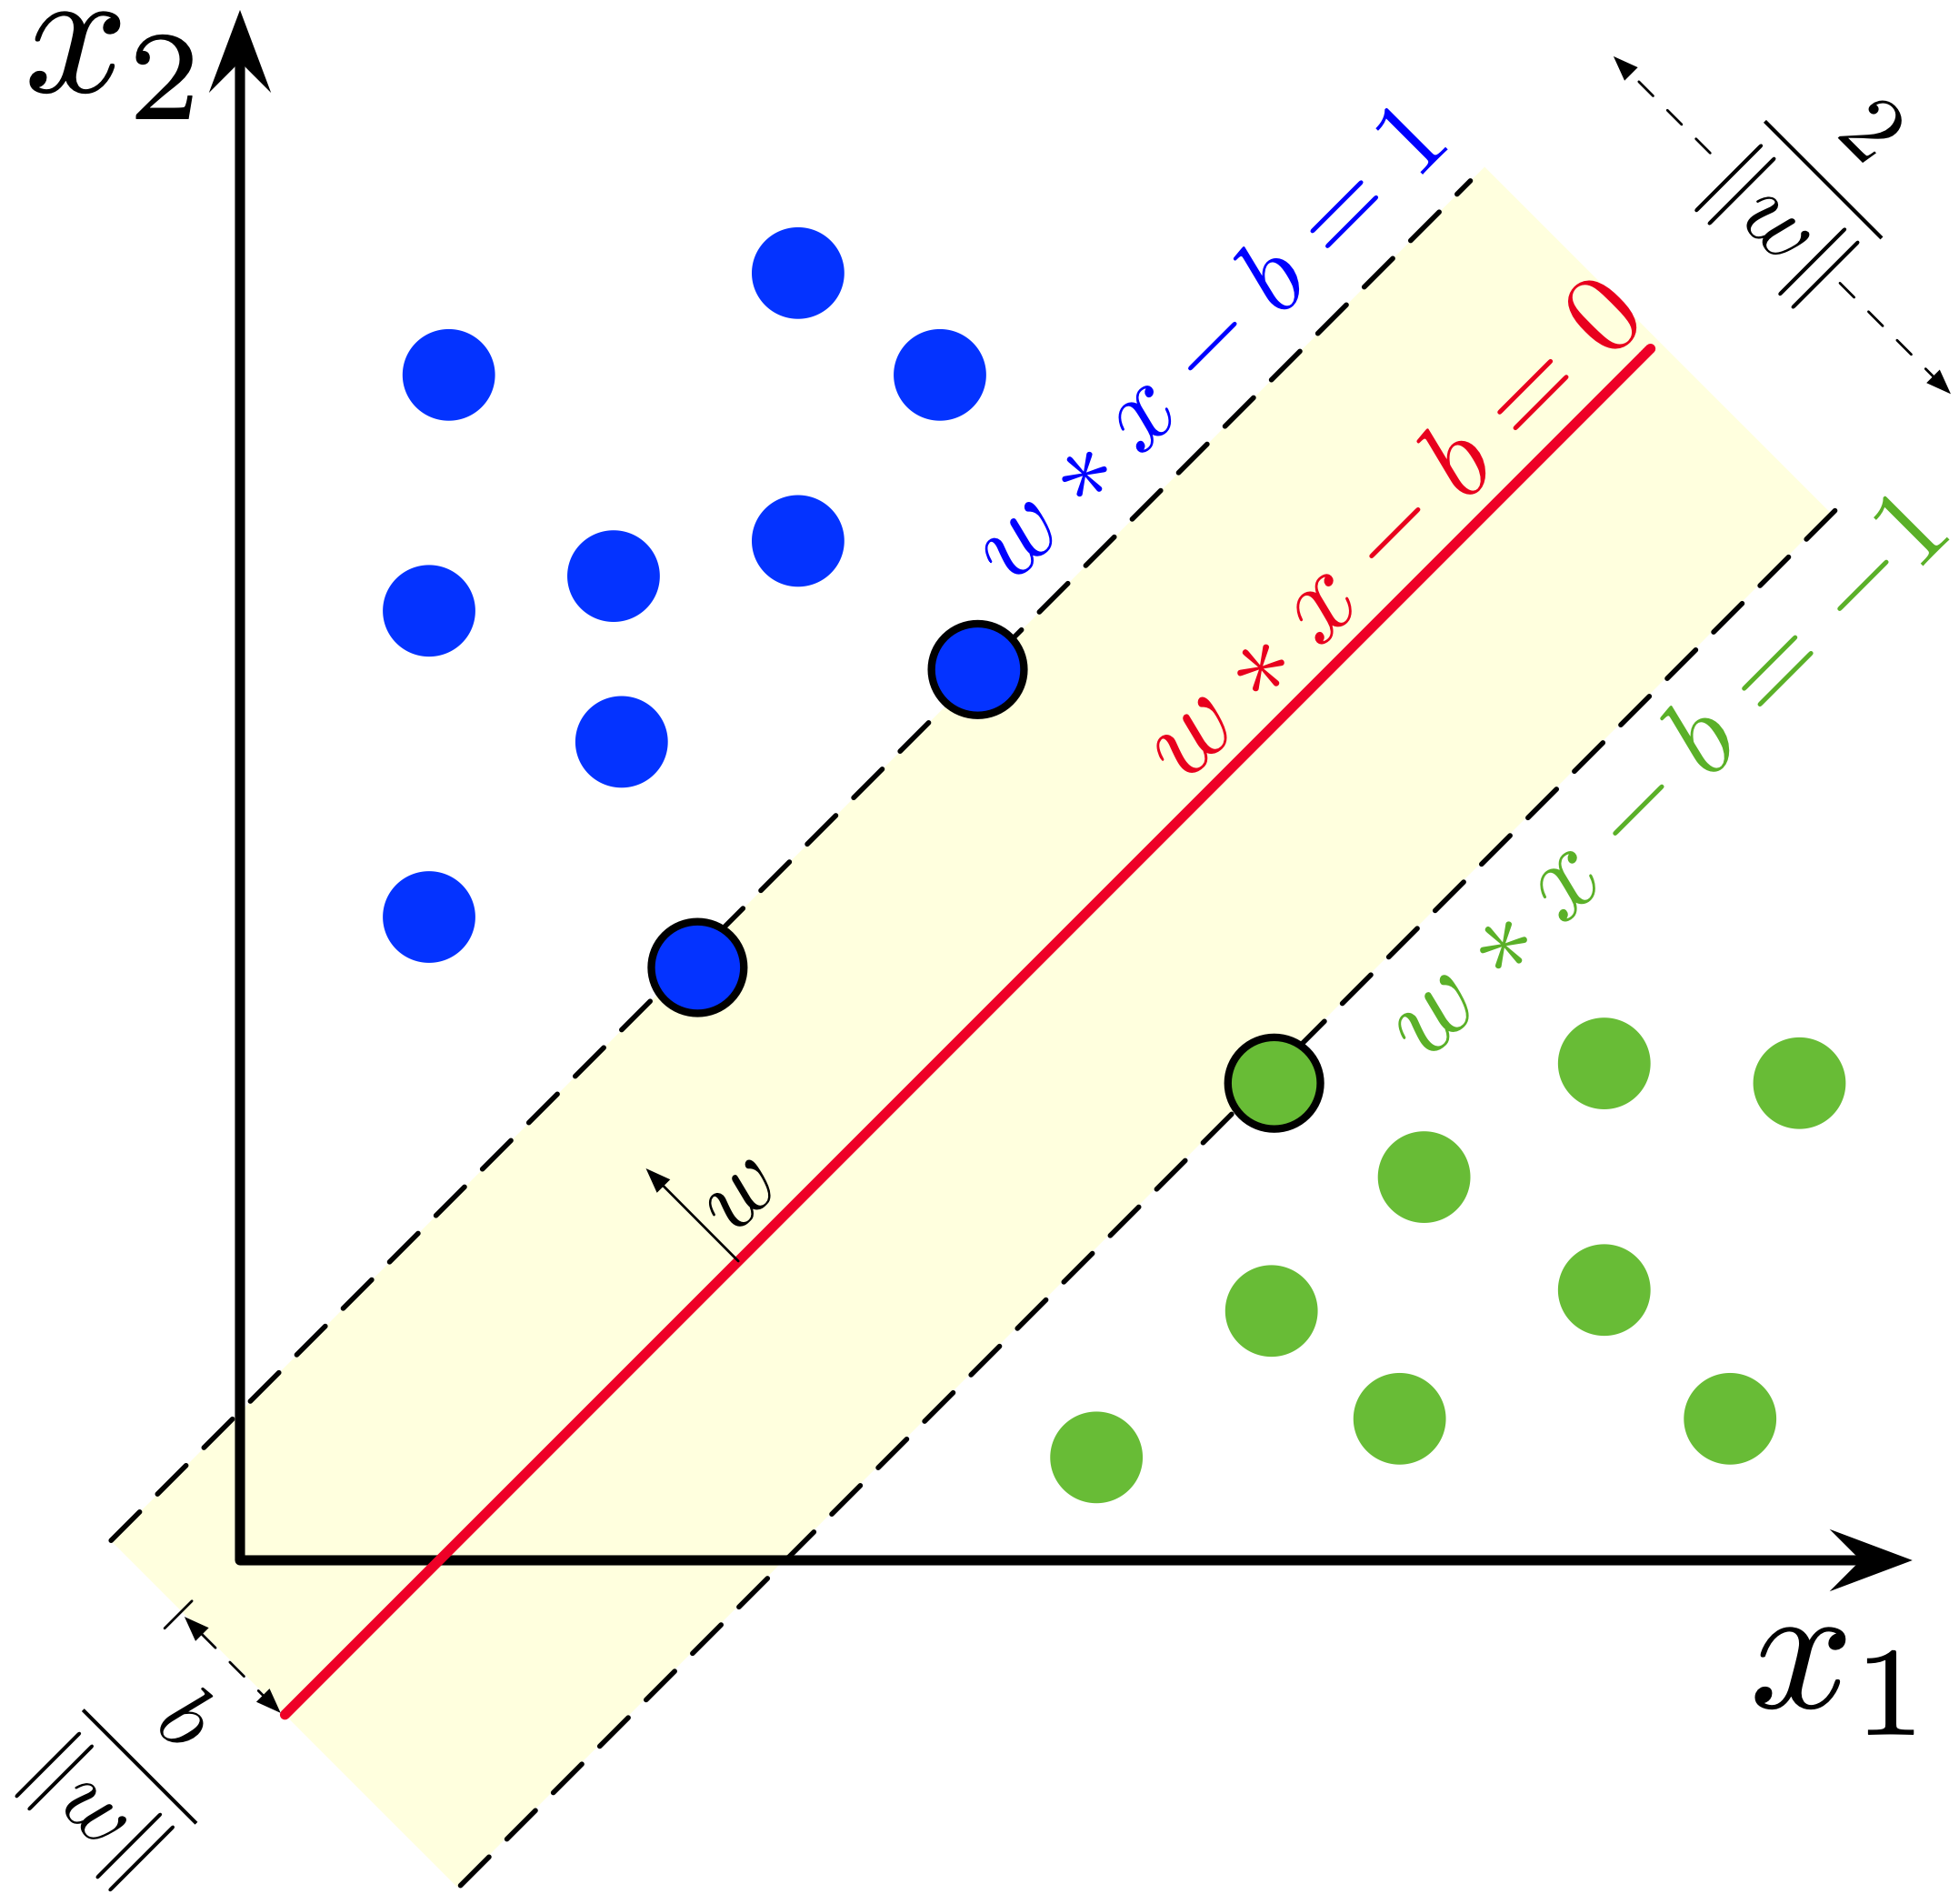
\includegraphics[width=.9\linewidth]{SVM_margin.png}
% 		\caption{linearly separable SVM}
% 	\end{subfigure}
% 	\begin{subfigure}{0.68\textwidth}
% 	\centering
% 		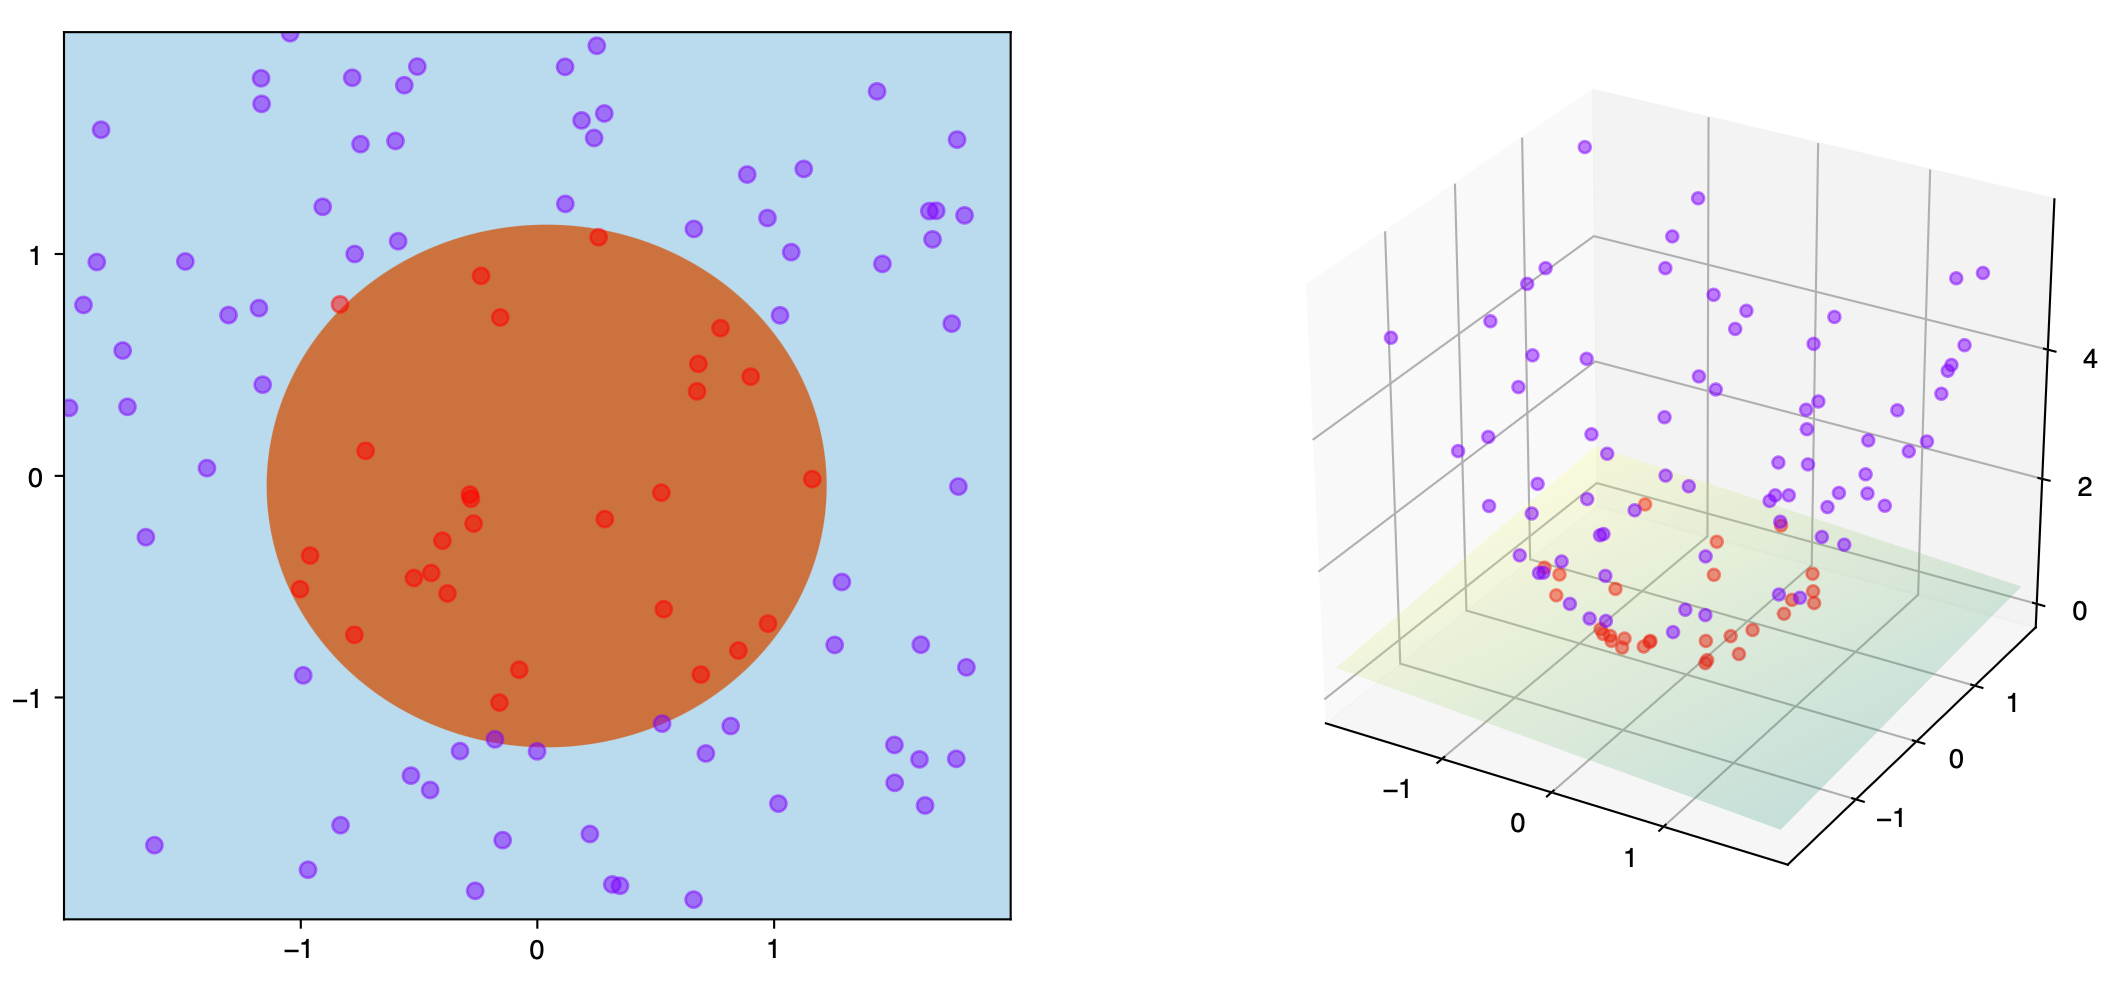
\includegraphics[width=.9\linewidth]{kernel_trick_idea.png}
% 		\caption{kernel trick idea: SVM with kernel given by $\phi(\vbx:=(a, b)) = (a, b, a^2 + b^2)$ and thus $\kernel(\vbx,\vb{y})=\vbx\cdot \vb{y}+\norm{x}^2 \norm{y}^2$ that only depends on inner product. The training points are mapped to a 3-dimensional space where a separating hyperplane can be easily found. (from Wikipedia: Kernel method)}	
% 	\end{subfigure}
% \end{figure}
\begin{figure}[!ht]
	\centering
	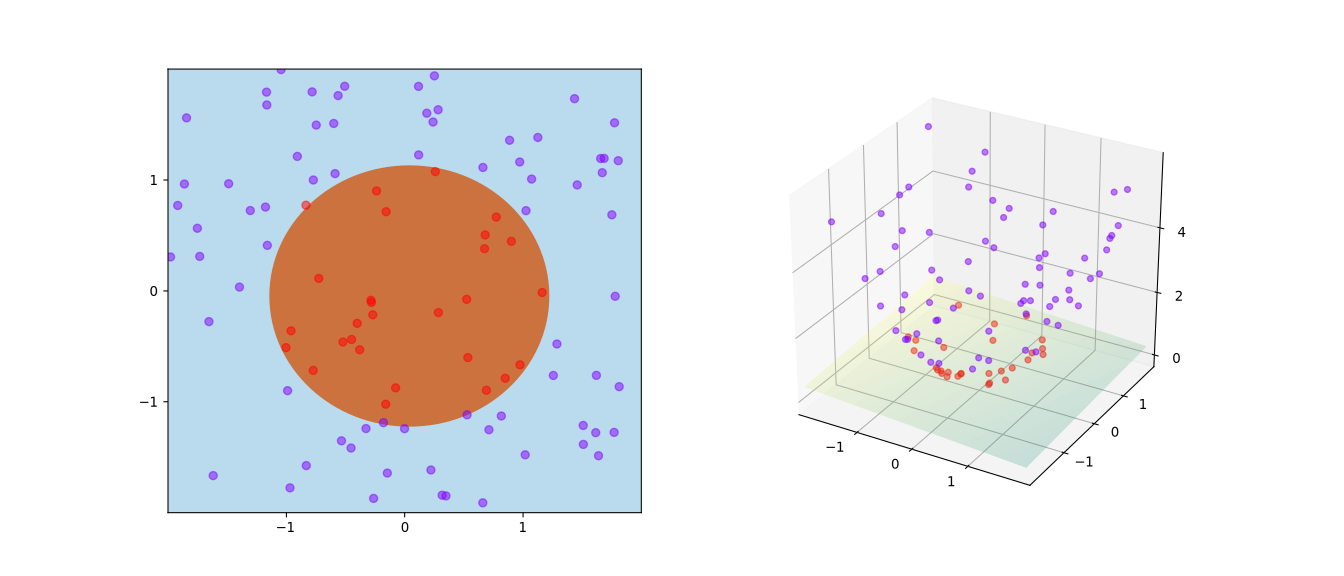
\includegraphics[width=0.6\linewidth]{Kernel_trick_idea.png}
	\caption{kernel trick idea: SVM with kernel given by $\phi(\vbx(x_1, x_2)) = (x_1, x_2, x_1^2 + x_2^2)$ and thus $\kernel(\vbx,\vbx')=\vbx\cdot \vbx' + \norm{\vbx}^2 \norm{\vbx'}^2$. The training points are mapped from a 2-dimensional to a 3-dimensional space where a separating hyperplane can be easily found. (from Wikipedia: Kernel method)}
	% that only depends on inner product
	\label{fig:kernel}
\end{figure}
Some common (popular) kernels on $\realnumber^d$ with dot product:
\begin{itemize}
	\item \emph{polynomial kernel}:
	$\kernel(\vbx,\vbx')=(c+\vbx\cdot \vbx')^p$.
	Take $d=2,p=2$ as an example, the corresponding feature map $\Phi(\vbx)=(x_1^2,x_2^2,\sqrt{2c}x_1,\sqrt{2c}x_2,c)^\T$.

	\item \emph{Gaussian (radial basis) kernel}:
	with the feature map $\Phi(\vbx)?=(\frac{1}{\sqrt{0!}}e^{-\vbx^2}\vbx^0,\dots,\frac{1}{\sqrt{n!}}e^{-\vbx^2}\vbx^n,\dots)$ (infinite dimensions)
	\begin{equation}
		\kernel(\vbx,\vbx') = 
		\exp(-\frac{\norm{\vbx-\vbx'}^2}{2\sigma^2})
		% =?
		\label{eq:gaussian_kernel}
	\end{equation}
	% \item Radial Kernels (Ornstein Uhlenbeck):
	% \begin{equation}
	% 	\kernel(\vbx,\vbx') = 
	% 	\exp(-\frac{\norm{\vbx-\vbx'}}{\gamma})
	% \end{equation}
\end{itemize}
Note that the Hilbert space associated with the Gaussian RBF kernel has infinite dimension, but the kernel may be readily computed for any pair of data points.
The kernel only depends on the inner product $\vbx\cdot\vbx'$ (without calculating the feature map explicitly). 
% we don't need the explicit mapping $\Phi$ as the kernel alone defines the solution 
graph kernels discuss in the remainder of this paper.

\begin{definition}[Reproducing Kernel Hilbert Space]\label{def:rkhs}
	It is well known that any continuous, symmetric, positive definite (\nameref{def:kernel}) has corresponding Hilbert space $\hilbertspace$ of (any real) functions $f$ defined on $\inputspace$, 
	called the \emph{Reproducing Kernel Hilbert Space} (RKHS) with the \emph{reproducing property}
	\begin{equation}
		f(\vbx) = \expval{f(\cdot),\kernel(\cdot,\vbx)}
	\end{equation}
	% which induces a \nameref{def:feature_map_classical} satisfying \cref{eq:kernel_classical}.
\end{definition}
% \begin{theorem}[Representer theorem]
% 	the kernel trick ? or more formally the \emph{representer theorem}
% 	\cite{chatterjeeGeneralizedCoherentStates2017}
% \end{theorem}

\section{Graph Kernels and Quantum Random Walks}
We commence by reviewing the classical graphs kernels and quantum random walks.
Largely, this development was driven by the empirical success of supervised learning of vector-valued data or image data. However, in many domains, such as chemo- and bioinformatics, social network analysis or computer vision, observations describe relations between objects or individuals and cannot be interpreted as vectors or fixed grids; instead, they are naturally represented by graphs.
\cite{kriegeSurveyGraphKernels2020}
graph-structured data is to make use of graph kernels—functions which measure the similarity between graphs.
\textbf{How similar are two graphs?}
\textbf{How similar are two nodes of a graph?}

\subsection{Diffusion kernel of a pair of vertices}
\cite{kondorDiffusionKernelsGraphs2002}.
generalize to regularization \cite{kondorGraphletSpectrum2009}: 
We propose a family of regularization operators (equivalently, kernels) on graphs that include Diffusion Kernels as a special case, and show that this family encompasses all possible regularization operators invariant under permutations of the vertices in a particular sense.
\cite{smolaKernelsRegularizationGraphs2003}
with Euclidean space $\Omega = \realnumber^m$

\begin{definition}[Adjacency matrix]\label{def:adjacency_matrix}
	Given a (undirected, unweighted) graph $\graph(V,E)$, its \emph{adjacency matrix} $\hat{A}$ is defined as
	\begin{equation}
		\hat{A}_{v,v'} : = 
		\begin{cases}
			1, & (v,v') \in E \\
			0, & \text{otherwise}
		\end{cases}
	\end{equation}
	where the matrix entry is 1 if the two vertices $v,v'$ (labels of the column and the row) are connected by an edge, otherwise the entry is 0.
\end{definition}
\begin{definition}[Graph Laplacian]\label{def:graph_laplacian}
	With the adjacency matrix $\hat{A}$, the graph Laplacian is obtained by
	\begin{equation}
		\llaplacian:=\hat{A}-\hat{D}	
		% \Longleftrightarrow
		% \hhat_0=\frac{\phat^2}{2m}
		% % \sim \nabla^2
		% =-\frac{\hbar^2\nabla^2}{2m}
		% % \Longleftrightarrow \dlagrangian ?
	\end{equation}
	where $\hat{D}_{v,v}:=\textup{deg}(v)=\sum_{v}[\hat{A}]_{v,v'}$ is the diagonal degree matrix.
\end{definition}
	Analogously, the adjacency matrix and graph Laplacian of weighted graphs can be defined.
% \begin{remark}
	Graph Laplacian $\llaplacian$ is the 
	discrete version of (continuous) Laplacian operator $\laplacian$
	\cite{chungSpectralGraphTheory1997}.
% \end{remark}
\begin{observation}
	The matrix exponential of any ? $\hhat$ i.e., $e^{\beta \hamiltonian}$, is a valid kernel (PSD). [to verify for $e^{-\ii t\hamiltonian}$]
\end{observation}
The diffusion kernel is defined as the exponential of the generator (Laplacian)
\begin{definition}[Diffusion kernel]\label{def:diffusion_kernel}
	The \emph{diffusion kernel} of a graph w.r.t a pair of vertices $(v,v')$ is
	% \cite{kondorDiffusionKernelsGraphs2002}
	% is $\kernel(v,v'):V(G)\to \realnumber$, i.e.,
	\begin{equation}
		\kernel(v,v') := 
		\qty[\sum_{k}\frac{\beta^k}{k!}\llaplacian^k]_{v,v'}  =
		\qty[e^{\beta \llaplacian}]_{v,v'} 
	\end{equation}
	where the input space $\inputspace$ is the set of vertices $V$ of graph $G$.
\end{definition}

\subsubsection{Diffusion, heat equation, and random walk}
The continuous-time random walk on $G$ is defined as the \textbf{solution of the differential equation}
\begin{equation}
	\dv{t} p_j(t)
	=
	\sum_{k\in V} \llaplacian_{jk} \ p_k(t),
	\label{eq:continuous_time_random_walk}
\end{equation}
where $p_j(t)$ denotes the probability associated with vertex $j$ at time $t$
and $\llaplacian$ is \nameref{def:graph_laplacian}.
Since the columns of $\llaplacian$ sum to 0,
% \begin{equation}
% 	\dv{t} \sum_{j\in V} p_j (t) = 
% 	\sum_{j,k\in V} \llaplacian_{jk}  p_k(t) = 0
% \end{equation}
% which shows that 
an initially normalized distribution remains normalized:
the evolution of the continuous-time random walk for any time $t$ is a \emph{stochastic process}.
\emph{random walk} (discrete-space, discrete-time), 
discretize the time derivative in \cref{eq:continuous_time_random_walk}
\begin{equation}
	p_j(t+1) = \frac{p_{j+1}(t) + p_{j-1}(t)}{2} 
\end{equation}
which is the finite difference equation of \emph{heat equation} 
\begin{equation}
	\pdv{p(t,x)}{t} = \pdv{ ^2 p(t,x)}{x^2}
	% u_t = \alpha \laplacian u \equiv \alpha \Delta u
	\label{eq:heat_equation}
\end{equation}
continuous-space (continous-time) case.
The solution to \cref{eq:heat_equation} is called \emph{heat kernel} $\kernel(t;x,x')=\frac{1}{4\pi t} e^{-\abs{x-x'}^2/4t}$ (Gaussian).

\subsection{Continuous-time quantum random walk}\label{sec:ct_quantum_walk}
These properties result in an exponential increase of the dimensionality of the state-space, which is the basis of the quantum speedup.
The continuous-time quantum random walk \cite{childsExampleDifferenceQuantum2002} is the quantum analogue of classical diffusion (continuous-time random walk).
By a direct observation, \cref{eq:continuous_time_random_walk} is very similar to the time-dependent (evolution) schrodinger equation governed by a Hamiltonian operator $\hamiltonian$
\begin{equation}
	\ii\hbar \dv{t} \ket{\psi} = \hamiltonian \ket{\psi}
	\label{eq:evolution}
\end{equation}
except that the factor of $\ii\hbar$.
\begin{definition}[Quantum propagator]\label{def:quantum_propagator}
	\emph{Quantum propagator} is a function that specifies the probability amplitude for a particle to travel from one place to another in a given period of time.
	This propagator may also be written as the \emph{transition amplitude}.
	\begin{equation}
		\kernel (x,t;x',t')
		=
		\mel{x}{e^{-\ii t \hamiltonian}}{x'}
		=
		\mel{x}{\U}{x'}
	\end{equation}
\end{definition}
Interestingly, this quantity is also called \emph{quantum kernel} (much earlier than the concept of kernel tricks in machine learning).
The propagator of a one-dimensional free particle can be evaluated 
\begin{equation}
	\kernel_{free}(x_I,0;x_F,t)  =
	\mel{x_F}{e^{-\ii t \phat^2/(2m\hbar) }}{x_I}
    =
	\sqrt{\frac{m}{2\pi \ii \hbar t}}
    \exp(\frac{\ii}{\hbar}\frac{m (x_F-x_I)^2}{2t}).
    \label{eq:free_propagator}
\end{equation}
by \emph{path integral (Lagrangian) formalism} (see \cref{sec:lagrangian}).
It is Gaussian form again.

\subsection{Graph kernels of a pair of graphs}
R-convolution kernel proposed by Haussler \cite{hausslerConvolutionKernelsDiscrete1999}.
graphs kernels are designed to compare the similarity of each of the decompositions of a pair of graphs.
Different kernels are defined, depending on how the graphs are decomposed.
Most R-convolution kernels count the number of isomorphic substructures in the two graphs.
random walk kernel (shortest paths)
\cite{vishwanathanGraphKernels2010}. 
quantum kernel
\cite{baiQuantumJensenShannon2015}
survey
\cite{kriegeSurveyGraphKernels2020}
\begin{definition}[Graph kernel]\label{def:graph_kernel}
	Given a pair of graphs $(G,G')$,
	a \emph{graph kernel} is a function (mapping)
	$\kernel(G,G'): \qty{ \graph } \to \realnumber$
	\begin{equation}
		\kernel(G,G') =
		\frac{1}{\abs{G}\abs{G'}}
		\sum_k \frac{\lambda^k}{k!} \vbe^\T A_{\times} \vbe
		=\frac{1}{\abs{G}\abs{G'}}
		\vbe^\T \exp(\beta \hat{A}_{\times}) \vbe
	\end{equation}
	\emph{random walk kernel} ?
\end{definition}
% \cite{chungSpectralGraphTheory1997}
\begin{definition}[Products of graphs]\label{def:product_graphs}
	The \emph{direct product of graphs}, 
	$G_{\times}(V_{\times},E_{\times}) : =G(V,E)\times G'(V',E') $
	\begin{equation}
		V_{\times}:= \qty{(v,v')\in V\times V'}
		,\quad
	% \end{equation}
	% \begin{equation}
		E_{\times}:= \qty{\qty((v_i,v_i'),(v_j,v_j'))\subseteq V_{\times}\times V_{\times}: (v_i,v_j)\in E \wedge (v_i',v_j')\in E'}
	\end{equation}
	where $V\times V'$ is the Cartesian product of two sets.
	% \begin{equation}
	% 	G_{\times} 
	% 	% : =	G(V,E)\times G'(V',E') 
	% 	: = \qty{(v,v')\in V\times V',((v,v'),(w,w')): (v,w)\in E, (v',w')\in E'}
	% \end{equation}
	\begin{itemize}
		\item 
	\emph{tensor (Kronecker) product of graphs}; $G\otimes G' := \qty{ \vee }$
	% \begin{equation}
	% 	G\otimes G' := \qty{ \vee }
	% \end{equation}
		\item 
	\emph{Cartesian product of graphs}; $G\times G' = \qty{}$
	% \begin{equation}
	% 	G\times G' = \qty{}
	% \end{equation}
		\item 
	% \emph{Kronecker sum};
	\emph{factor graph};
	% \emph{Hadamard product} element-wise multiplication;
	\end{itemize}
\end{definition}
\begin{fact}
	the adjacency matrix of the product graph $A_{\times}=A\otimes A'$ ($\exp(A_{\times}=\exp(A)\otimes \exp(A'))$).	
	In general, the Laplacian of the direct product graph 
	$\llaplacian_{\times}\neq \llaplacian_1\otimes \llaplacian_2$.
	Performing a random walk on the direct product graph is equivalent to performing a simultaneous random walk on G and G'.
\end{fact}
The idea of the shortest path kernel is to compare the attributes and lengths of the shortest paths between all pairs of vertices in two graphs.
\begin{definition}[Random walk kernel]
	\begin{equation}
		\kernel_{\times}(G,G) = 
	\end{equation}
\end{definition}
graph kernels based on random walks, which count the number of (label sequences along) walks that two graphs have in common.
% \begin{remark}
for diffusion processes on factor graphs the kernel on the factor graph is given by the product of kernels on the constituents, that is 
\begin{equation}
	\kernel((i, i'), (j, j')) = \kernel(i, j) \kernel' (i' , j' ).
\end{equation}
% \end{remark}
% \begin{remark}
Random Walk on Product Graph is equivalent to simultaneous random walk on input graphs [?]
% \end{remark}
\begin{remark}
	A natural question to ask is the following: Since diffusion can be viewed as a \textbf{continuous time} limit of random walks, can the ideas behind the random walk kernel be extended to diffusion? Unfortunately, the Laplacian of the product graph does not decompose into the Kronecker product of the Laplacian matrices of the constituent graphs; this rules out a straightforward extension.
	discrete-time quantum random walk (need coin space) \cite{ambainisCoinsMakeQuantum2005} \cite{childsQuantumInformationProcessing2004};
	Szegedy's walk formalism.
	\cite{szegedySpectraQuantizedWalks2004}
\end{remark}

\subsection{Discrete-time quantum random walk}
\emph{Discrete-time quantum random walk} is the quantum analogy of random walk
\cite{ambainisOnedimensionalQuantumWalks2001}.
\cite{baiQuantumKernelsUnattributed2017}

\subsection{Relations, difference, and examples}
\subsubsection{Line}
(classical) diffusion kernel of a 1-dimensional lattice (line)
\begin{equation}
	\kernel(v,v') = 
\end{equation}
\nameref{def:quantum_propagator} (quantum kernel)
\begin{align}
	\tilde{\kernel}(z_F,z_I) = 
	\mel{z_F}{e^{-\ii t\hhat_0 }}{z_I}
	&=\sum_{p=1}^{N} 
	e^{-\ii t 2\cos(\frac{2\pi}{N}p) +\ii \frac{2\pi}{N} p(z_I-z_F)} 
	\\
	&
	% \approx \frac{1}{2\pi} \int_{\pi}^{\pi} e^{\ii p d -2\ii t cos(p)} \dd{p} 
	\approx e^{2\ii t} (-\ii)^{d} J_{d} (2t)
	\tag{large N approx}
	\label{eq:ctqrw_kernel}
\end{align}
where the distance between .
\begin{figure}[!ht]
	\centering
	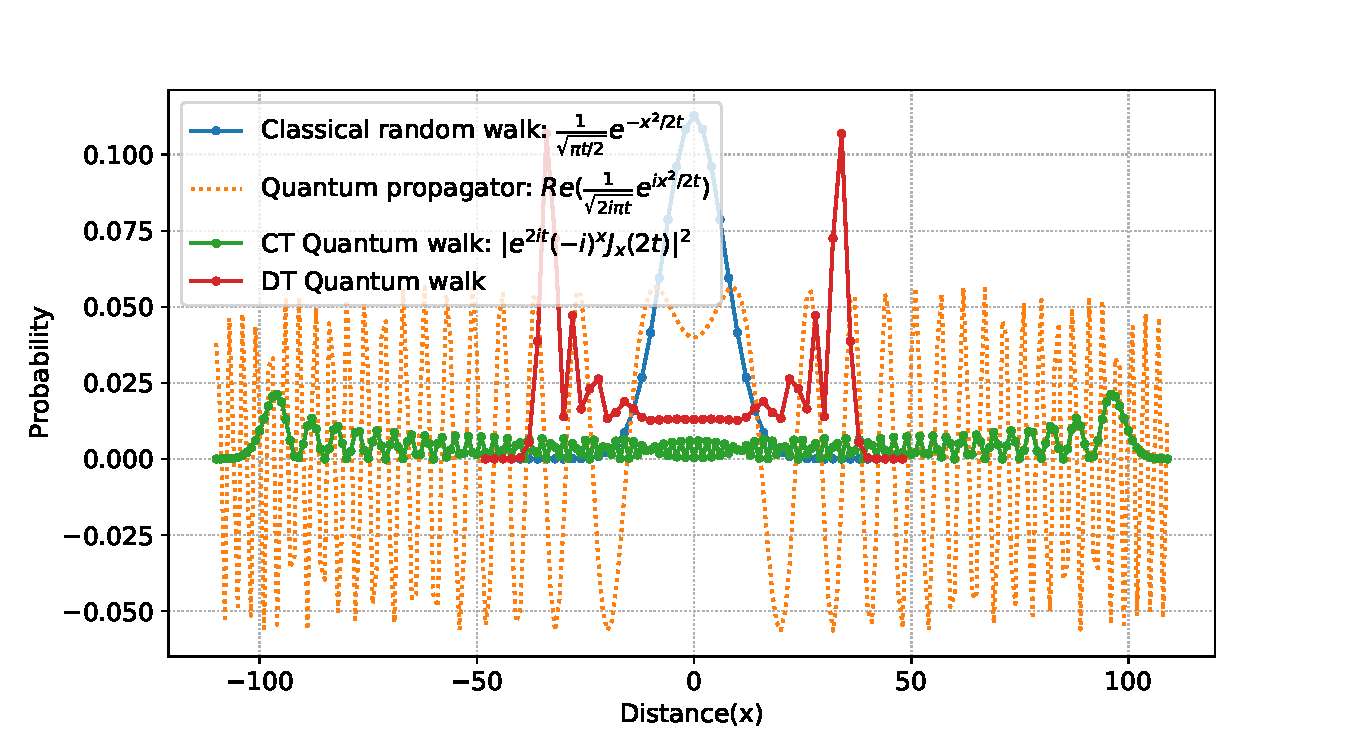
\includegraphics[width=.7\linewidth]{walk_propagator_1d.pdf}
	\caption{Different kinds of walks in 1d space}
\end{figure}
\begin{remark}
    The random walk on this graph starting from the origin (in either continuous or discrete time)
    typically moves a distance proportional to $\sqrt{t}$ in time $t$.
	In contrast, the quantum random walk spreads as a wave packet with speed 2.
\end{remark}

\subsubsection{Hyercube}
the unitary evolution operator of quantum diffusion on hypercube
\begin{equation}
	e^{-\ii t \hat{A}} = 
	\prod_{j=1}^n e^{-\ii t \px^{(j)} }
	= \bigotimes_{j=1}^n
	\begin{pmatrix}
		\cos t & -\ii \sin t \\ 
		-\ii \sin t & \cos t
	\end{pmatrix}
\end{equation}

\subsubsection{Tree (TODO)}

\subsubsection{Cayley graphs (TODO)}
\begin{definition}[Cayley graph]\label{def:cayley_graph}
	Cayley graph is a graph that encodes the abstract structure of a group. 
\end{definition}

\section{Quantum Advantages and Speedups}\label{sec:speedup}
provide both theoretical insight and numerical demonstrations for its success, and show its feasibility for near-term experimental implementation.
A quantum version of this approach has already been proposed in \cite{rebentrostQuantumSupportVector2014},
where an exponential improvement can be achieved if data is provided in a coherent superposition. 

% \subsection{Quantum Machine Learning: SVM and QKE}
\subsection{Related works}\label{sec:qke}
There have been several attempts to introduce kernel method to quantum machine learning.
% theoretically sound analogs of convolutional neural networks to quantum circuits, but they have generally been somewhat heuristic.
% is highly desirable because it not only helps to gain important physical insights about the system but also leads to more efficient

\subsubsection{Quantum SVM and kernel tricks}
Quantum version of SVM was proposed \cite{rebentrostQuantumSupportVector2014} to exploit the power of quantum computer.
, where an exponential improvement can be achieved if data is provided in a coherent superposition. However, when data is provided in the conventional way, i.e. from a classical computer, then the methods of [15] cannot be applied. \cite{tangQuantuminspiredClassicalAlgorithm2019}
% \cite{havlicekSupervisedLearningQuantum2019}
It is shown that a quantum support vector machine can be implemented with $O(\log md)$ run time in both training and classification stages. 
The performance in N arises due to a fast quantum evaluation of inner products.
For the performance in M, we re-express the SVM as an approximate least-squares problem [15] that allows for a quantum solution with the matrix inversion algorithm [16, 17]. We employ a technique for the exponentiation of non-sparse matrices recently developed in [18]. This allows us to reveal efficiently in quantum form the largest eigenvalues and corresponding eigenvectors of the training data overlap (kernel) and covariance matrices. We thus efficiently perform a low-rank approximation of these matrices (principal component analysis, PCA).
\begin{definition}[Quantum feature map]\label{def:quantum_feature_map}
	the quantum state space (Hilbert space) as the feature space to still obtain a quantum advantage
	mapping the input data non-linearly to a quantum state (density matrix) 
	\begin{equation}
		\Phi(\vbx): \Omega \to \dyad{\Phi(\vbx)},
		\label{eq:quantum_feature_map}
	\end{equation}
	the direct quantum analogy of classical \nameref{def:feature_map_classical}.
	On quantum computers, the quantum feature map $\Phi(\vbx)$ is realized by applying a unitary quantum circuit $\U_{\Phi(\vbx)}$ to a reference state $\ket{0^n}$.
\end{definition}
\begin{definition}[Quantum kernel estimation]\label{def:quantum_kernel}
	The \emph{quantum kernel estimation} is the \emph{Hilbert-Schmidt} \nameref{def:inner_product} between density matrices
	\begin{equation}
		\kernel(\vbx,\vbx') 
		= \Tr\qty(\dyad{\Phi(\vbx)}\cdot \dyad{\Phi(\vbx')})
		= \abs{\braket{\Phi(\vbx)}{\Phi(\vbx')}}^2 = 
		\abs{\matrixel{\vb{0}}{\U^\dagger_{\Phi(\vbx)} \U_{\Phi(\vbx')}}{\vb{0}}}^2.
	\end{equation}
	exactly the \nameref{def:quantum_propagator}.
\end{definition}
Naturally, the \emph{quantum kernel estimation}
\cite{schuldQuantumMachineLearning2019}
\cite{havlicekSupervisedLearningQuantum2019} 
is studied to enhance the performance of quantum SVM.
Here, we propose two SVM type classifiers that process data provided purely classically and use the quantum state space as the feature space to still obtain a quantum advantage.

\subsubsection{Quantum variational classification (explicit method)}
variational quantum circuit: generates a separating hyperplane in the quantum feature space.
the quantum variational classifier builds on \cite{mitaraiQuantumCircuitLearning2018} \cite{farhiClassificationQuantumNeural2018} and operates through using a variational quantum circuit to classify a training set in direct analogy to conventional SVMs.
not robust (heuristic)
To obtain an advantage over classical approaches we need to implement a map based on circuits that are hard to simulate classically.
% The exact evaluation of the inner-product between two states generated from a similar circuit with only a single diagonal layer is $\#P$ - hard.
\begin{enumerate}
	\item a classical datum $\vbx\in\Omega$ is mapped to a quantum (feature) state by applying a unitary circuit $\U_{\Phi(\vbx)}$ to a reference (initial) state $\ket{0}^n$
	\item a \textbf{short depth quantum} circuit $W(\pmb{\theta})$.
	iteratively optimize the circuit variational parameters $\pmb{\theta}$ 
	by minizing empirical error (cost function)
	\item for binary classification, apply a \textbf{binary measurement} in $Z$-basis
	% $\qty{M_y}=2^{-1}(\identity + y \vb{f})$?
	\item to obtain the empirical distribution $p_y(\vbx)$, perform repeated measurement shots.
	then assign the label according to $p_y$?
\end{enumerate}
hardness \cite{bremnerAveragecaseComplexityApproximate2016}.
the circuit is hard to simulate classically.
The hardness of estimating the kernel with classical resources is of course only a necessary and not always sufficient condition to obtain a quantum advantage.
% \begin{remark}
% 	While it may appear to be only a detail, it is important to define the feature state as the density matrix Φ(x).
% \end{remark}

\subsubsection{Quantum kernel estimation (implicit method)}
In this method, quantum computer is used only to estimate the kernel function (matrix).
implement a conventional (classical) SVM to generate the separating hyperplane
rather than using a variational quantum circuit.
% to generate the separating hyperplane, we use a classical SVM for classification.
% \begin{enumerate}
% 	\item the kernel $\kernel(\vbx,\vbx')$ is estimated on a quantum computer
% 	\item the quantum computer is used a second time to estimate the kernel for a new datum (test) $\vb{s}\in S$ with all the support vectors.
% \end{enumerate}

\textbf{The kernel entries are the fidelities between different feature vectors.}
The overlap can be estimated directly from the transition amplitude 
\namecref{def:quantum_kernel}.
measure the final state in the Z-basis R-times and record the number of $\ket{0^n}$.
The frequency of this string is the estimate of the transition probability.
The kernel entry is obtained to an additive sampling error of $\tilde{\epsilon}$ when $\bigO(\tilde{\epsilon}^{-2})$ shots are used.


\subsubsection{Quantum graph kernels}
quantum graph kernel defined in terms of quantum Jensen Shannon as a metric of dissimilarity of graphs
density matrices associated with (representing) the evolution of continuous-time quantum random walks on graphs
\cite{baiQuantumJensenShannon2015}.
In classical information theory, the Jensen-Shannon divergence is a similarity measure between probability distributions.
\begin{equation}
	D(p,p')
\end{equation}
\begin{remark}
	Unfortunately, the required composite entropy for the Jensen-Shannon kernel is computed from a product graph formed by a pair of graphs,
	and reflects no correspondence information between pairs of vertices.
	As a result, the Jensen-Shannon graph kernel lacks correspondence information between the probability distributions over the graphs,
	and thus cannot precisely reflect the similarity between graphs[??].
\end{remark}
Analogously, the quantum version of Jensen-Shannon divergence is defined as the distance measure between mixed quantum states (density matrices).
\begin{definition}[]
	Given a graph $\graph(V,E)$, the von Neumann entropy of $\graph$ is defined as
	\begin{equation}
		H_N (\rho_{\graph}) = -\Tr(\rho_{G}\log \rho_{\graph})
		= - \sum_{j}^{\abs{V}} \lambda_j \log \lambda_j
	\end{equation}
	where $\rho_{\graph}$ is .. and $\lambda$ is ....
	Given two density operators $\rho$ and $\rho'$,
	the \emph{quantum Jensen-Shannon divergence} is defined as
	\begin{equation}
		D_{QJS} (\rho,\rho') = 
		H_N\qty(\frac{\rho+\rho'}{2}- \frac{1}{2}H_N(\rho)) - \frac{1}{2} H_N (\rho')
	\end{equation}
	$D_{QJS}$ is always well defined, symmetric, negative definite and bounded, i.e., $0\le D_{QJS}\le 1$?.
\end{definition}
PSD?

\subsubsection{Quantum diffusion map}
Inspired by random walk on graphs, \emph{diffusion map} (DM) is a class of \textbf{unsupervised} machine learning that offers automatic identification of \textbf{low-dimensional data structure hidden in a high dimensional dataset}.
Though both of SVM and DM are machine learning techniques that utilize kernel tricks, DM is designed for dimension reduction, the `reverse direction' of the kernel trick in SVM.
Like other dimension reduction technique, DM entails the calculate the eigenvalue/vectors (SVD).
% Most dimensionality reduction methods require the computation of singular value decomposition (SVD) of a matrix constructed from a collection of high-dimensional data points. $\bigO(N^3)$
Thus, classical dimensionality reduction can be computationally prohibitive for a large data sample. 
However, under moderate assumptions of accessibility to certain features of full-scale quantum computers, matrix exponentiation-based quantum algorithms have been proposed to perform SVD more efficiently [17]. 
% \begin{remark}
% 	Although the backbone of DM is a graph-based dimensionality reduction method, the procedure is different from other spectral graph methods. 
% 	Namely, rather than working with the data-induced graph Laplacian as in Laplacian eigenmaps or in spectral clustering, DM involves Markov transition matrix that defines random walks on a data-induced graph.
% \end{remark}
The quantum diffusion map (qDM) consists of 5 major steps: 
\begin{enumerate}
	\item \nameref{def:coherent_state} data encoding scheme, 
	\item 
	a natural construction of kernel matrix from coherent states, 
	\cref{eq:diffusion_map_kernel}
	\item 
	a scheme to construct the Markov transition matrix from the kernel matrix, 
	\item 
	the eigen-decomposition of the transition matrix (quantumly $\bigO(\poly\log N)$?); classical $\bigO(m^3)$
	\item 
	and extracting relevant quantum information to construct diffusion map classically. 
	and classically constructs the diffusion map via the readout (tomography) of the eigenvectors, giving a total expected runtime proportional to $N^2 \poly\log N$.
\end{enumerate}
The expected time complexity of qDM is $N^2 \poly\log N$, compared to the worst-case runtime $\bigO(N^3 )$ of a classical DM. 
Importantly, from accessing of qRAM to performing an eigendecomposition of the Markov transition matrix, the total time complexity is only $\bigO(\log^3 N)$.
Given the normalized (similarity) matrix $M$, 
compute the $k$ largest eigenvalues(vectors) of $M^t$.
Rather than using mere Euclidean distance as a similarity measure between data points, manifold learning approach assigns the connectivity among data points in their neighborhood as a proxy for proximity between points.
% \begin{remark}
% 	Two points whose squared distance exceed this bandwidth contribute exponentially little to the weighted edge, suggesting that these two points are far away from being a neighbor in its original feature space.
% \end{remark}
In DM, the similarity matrix between a pair of data vectors, or equivalently the weighted edge between a pair of graph vertices, is often taken to be a Gaussian kernel \cref{eq:gaussian_kernel}:
\begin{equation}
	W_{ij}:=\kernel (\vbx^{(i)},\vbx^{(j)}) =
	\exp(-\frac{\norm{\vbx^{(i)}-\vbx^{(j)}}_2^2}{2\sigma})
	\label{eq:diffusion_map_kernel}
\end{equation}
where the adjustable parameter $\sigma$, called the bandwidth, sets the scale of neighborhood.
Given a graph with weighted edges $W_{ij}$ ’s, DM assigns a \emph{discrete-time random walk} on a data-induced graph, 
where the Markov transition probability from vertex $i$ to $j$ is given by the normalized weighted edge,
\begin{equation}
	P_{ij} = \frac{W_{ij}}{\sum_{j}W_{ij}}
	,
	P = D^{-1} W
\end{equation}
% \begin{remark}
% 	The notion of proximity based on graph connectivity can be characterized by how fast random walkers on a graph starting at different data points visit each other. One expects that two points that are connected by multiple paths should be near; whereas two points that are sparsely connected should lie far from each other.
% \end{remark}
Use the diffusion map to get the embedding $\Psi_t$.
% \begin{equation}
% 	P, L
% \end{equation}
\begin{definition}[Coherent state]\label{def:coherent_state}
	A \emph{coherent state} is ...
	\begin{equation}
		\ket{\alpha} 
		% = \sum_{n=0}^{\infty} \ket{n} \braket{n}{\alpha}
		= e^{-\frac{1}{2}\abs{\alpha}^2} \sum_{n=0}^{\infty} \frac{\alpha^n}{\sqrt{n!}} \ket{n} 
		= e^{-\frac{1}{2}\abs{\alpha}^2} e^{\alpha\acreation}\ket{0} 
	\end{equation}
	where $\ket{n}$ basis and $\acreation$ is the creation operator [ref].
	% displacement operator
	% \begin{equation}
	% 	\hat{D}(\alpha)\ket{0} : = e^{\alpha \acreation - \alpha^* \aannihilation} \ket{0} = \ket{\alpha}
	% \end{equation}
\end{definition}
Consider two $n$ tensor product of (canonical) coherent states
\begin{equation}
	\ket{\pmb{\alpha}} = \ket{\alpha_{1}} \otimes\ket{\alpha_{2}} \cdots\otimes\ket{\alpha_{n}} 
	,\quad
	\ket{\pmb{\alpha}'} = \ket{\alpha_{1}'} \otimes\ket{\alpha_{2}'} \cdots\otimes\ket{\alpha_{n}'} 
\end{equation}
with $\vbx=(\alpha_1,\alpha_2,\dots,\alpha_n)$ and $\vbx'=(\alpha_1',\alpha_2',\dots,\alpha_n')$, the kernel reads
\begin{equation}
	\abs{\braket{\pmb{\alpha}}{\pmb{\alpha}'}}^2 = 
	\exp(-\norm{\vbx-\vbx'}^2) 
\end{equation}
which is the Gaussian kernel c.f. \cref{eq:gaussian_kernel} and \cref{eq:diffusion_map_kernel}.
One of the most significant limitations of classical algorithms using non-linear kernels is that the kernel function has to be evaluated for all pairs of input feature vectors which themselves may be of substantially high dimension. [quantum parallelism (superposition) measurement]
The key link will be the \nameref{def:rkhs} property for SVMs that naturally arise from canonical and generalized coherent states. 
Specifically, we discuss the fast evaluation of radial kernels through a positive operator valued measure (POVM) on a quantum optical system based on canonical coherent states.
\cite{chatterjeeGeneralizedCoherentStates2017}
The quantum DM proposed by \cite{sornsaengQuantumDiffusionMap2021} takes as an input $N$ classical data vectors, 
performs (quantumly) an eigen-decomposition of the Markov transition matrix in time $\bigO(\log^3 N)$, 


\subsection{Provable quantum speedups}
structure is required for quantum speedup
\cite{aaronsonNeedStructureQuantum2014}.
only polynomial speedup for total problem [ref].
only quadratic speedup for unstructured search \cite{groverQuantumMechanicsHelps1997}
the core challenge to provable quantum speedup and practical problems.

\subsubsection{Quantum linear algebra toolbox (subroutines)}
\cite{sornsaengQuantumDiffusionMap2021}
\emph{Fast Fourier Transform}  (FFT) \cite{kondorGraphletSpectrum2009};
quantum linear algebra (qMAT) \cite{zhaoCompilingBasicLinear2019}: 
\begin{itemize}
	\item HHL quantum algorithm for linear equation systems \cite{harrowQuantumAlgorithmSolving2009}, qSVD (eigen decomposition) [ref]
	\item matrices multiplication, matrix inversion, matrix exponentiation, 
	\item quantum simulation techniques (evolution); QFT, quantum phase estimation.
	\item FFT by quantum algorithms: $\bigO(n\log n)$; 
	It is shown that quantum circuits are a natural choice for Fourier space neural architectures affording a super-exponential speedup in computing the matrix elements of $\mathbb{S}_n$-Fourier coefficients compared to the best known classical (FFT) over the symmetric group. \cite{zhengSpeedingLearningQuantum2022}
\end{itemize}

\subsubsection{Quantum Fourier Transform (QFT) and algebraic problems}
hidden subgroup problem solved by quantum Fourier transformation\cite{childsQuantumAlgorithmsAlgebraic2010};
rigorous and robust quantum speedup with Discret Logarithm problem \cite{liuRigorousRobustQuantum2021} \cite{glickCovariantQuantumKernels2021}
\begin{problem}[Hidden subgroup problem]\label{prm:hidden_subgroup}
	Given a group $\group$ and a black-box function $f:\group\to S$, 
	$f$ is promised to satisfy 
	\begin{equation}
		f(x) =f(y) \iff x^{-1}y \in \subgroup 
	\end{equation}
	for some unknow subgroup $\subgroup \le \group$.
	We say such a function $f$ hides a subgroup $\subgroup$.
	The goal of \emph{hidden subgroup problem} (\hsp) is to learn $\subgroup$
	(specified in terms of a generating set) using queries to $f$.
\end{problem}
\begin{remark}
	Simon's problem [ref] 
	% (Abelian subgroup problem) 
	is a $\hsp$ with $\group = \integer^n_2$ and $\subgroup = \qty{ 0, s }$ for some $s \in \integer_2^n$ .
\end{remark}
% robust, provable speedup \cite{liuRigorousRobustQuantum2021}
\begin{problem}[Discrete Logarithm problem]\label{prm:dlog}
	The \emph{discrete logarithm problem} (\dlog) is defined as
	\begin{itemize}
		\item \textbf{Input:} a prime $p$, a primitive element (generator) $g$ of $\integer_p^*=\qty{1,2,\dots,p-1}$, and an element $y=g^x \pmod{p} \in\integer_p^*$ with some unknow $x$. black-box function $f$?
		\item \textbf{Output (goal):} find $x=\log_g y$
	\end{itemize}
	$\dlog$ is a special case of $\hsp$ with ... subgroup 
\end{problem}
reducible to decision version $\dlog_{1/2}$, then classification version.
\begin{equation}
	\dlog \le \dlog_{1/2} \le \dlog
\end{equation}
$\le$ represents polynomial (time) reduction.

covariant quantum kernels for the data with group structures
\cite{glickCovariantQuantumKernels2021}
The feature states are intimately related to covariant measurements?
Examples could constitute learning permutations or classifying translations or rotations. Exploiting group structure and learning problems for group data have already been investigated for classical kernels \cite{kondorGraphletSpectrum2009}.
The fiducial state $\ket{\phi}$ is chosen as some reference state from the representing Hilbert space. 
In principle, any state that can be prepared efficiently may be chosen. 
However, the choice will greatly affect the performance of the classifier as we will discuss shortly.
\begin{definition}[Covariant]\label{def:covariant}
	\emph{covariant}
	feature map circuits that we call covariant feature maps. 
\end{definition}
kernel alignment?
\begin{problem}[labeling cosets with error]
	\emph{labeling cosets with error}

	\begin{itemize}
		\item 
		\textbf{Input:} given a group $\group$ and subgroup $\subgroup$,
		we can define two left-cosets $\mathbb{C}_{\pm}=c_{\pm}\subgroup$ by choosing $c_+,c_-$ randomly

		\item 
		\textbf{Output: ?} 
	\end{itemize}

	% this problem is related to the problem of deciding membership in a subgroup
\end{problem}

\subsubsection{Permutation, symmetry, and graph properties}
fully symmetric (partial) functions do not admit exponential quantum speedup in the query model.
\cite{ben-davidSymmetriesGraphProperties2020}.
\begin{problem}[Glued tree]
	see \cref{fig:glued_tree}
	\begin{itemize}
		\item \textbf{Input:} a glued tree in the \nameref{def:adjacency_matrix} representation, oracle (neighbor)?
		\item \textbf{Output (goal):} find the exit (start from entrance)
	\end{itemize}
\end{problem}
Consider a graph obtained by starting from two balanced binary trees of height n, and joining them by a random cycle of length $2\cdot 2^n$ that alternates between the leaves of the two trees. 
For example, such a graph for $n = 4$ could look like \cref{fig:glued_tree}
\begin{figure}[!ht]
	\centering
	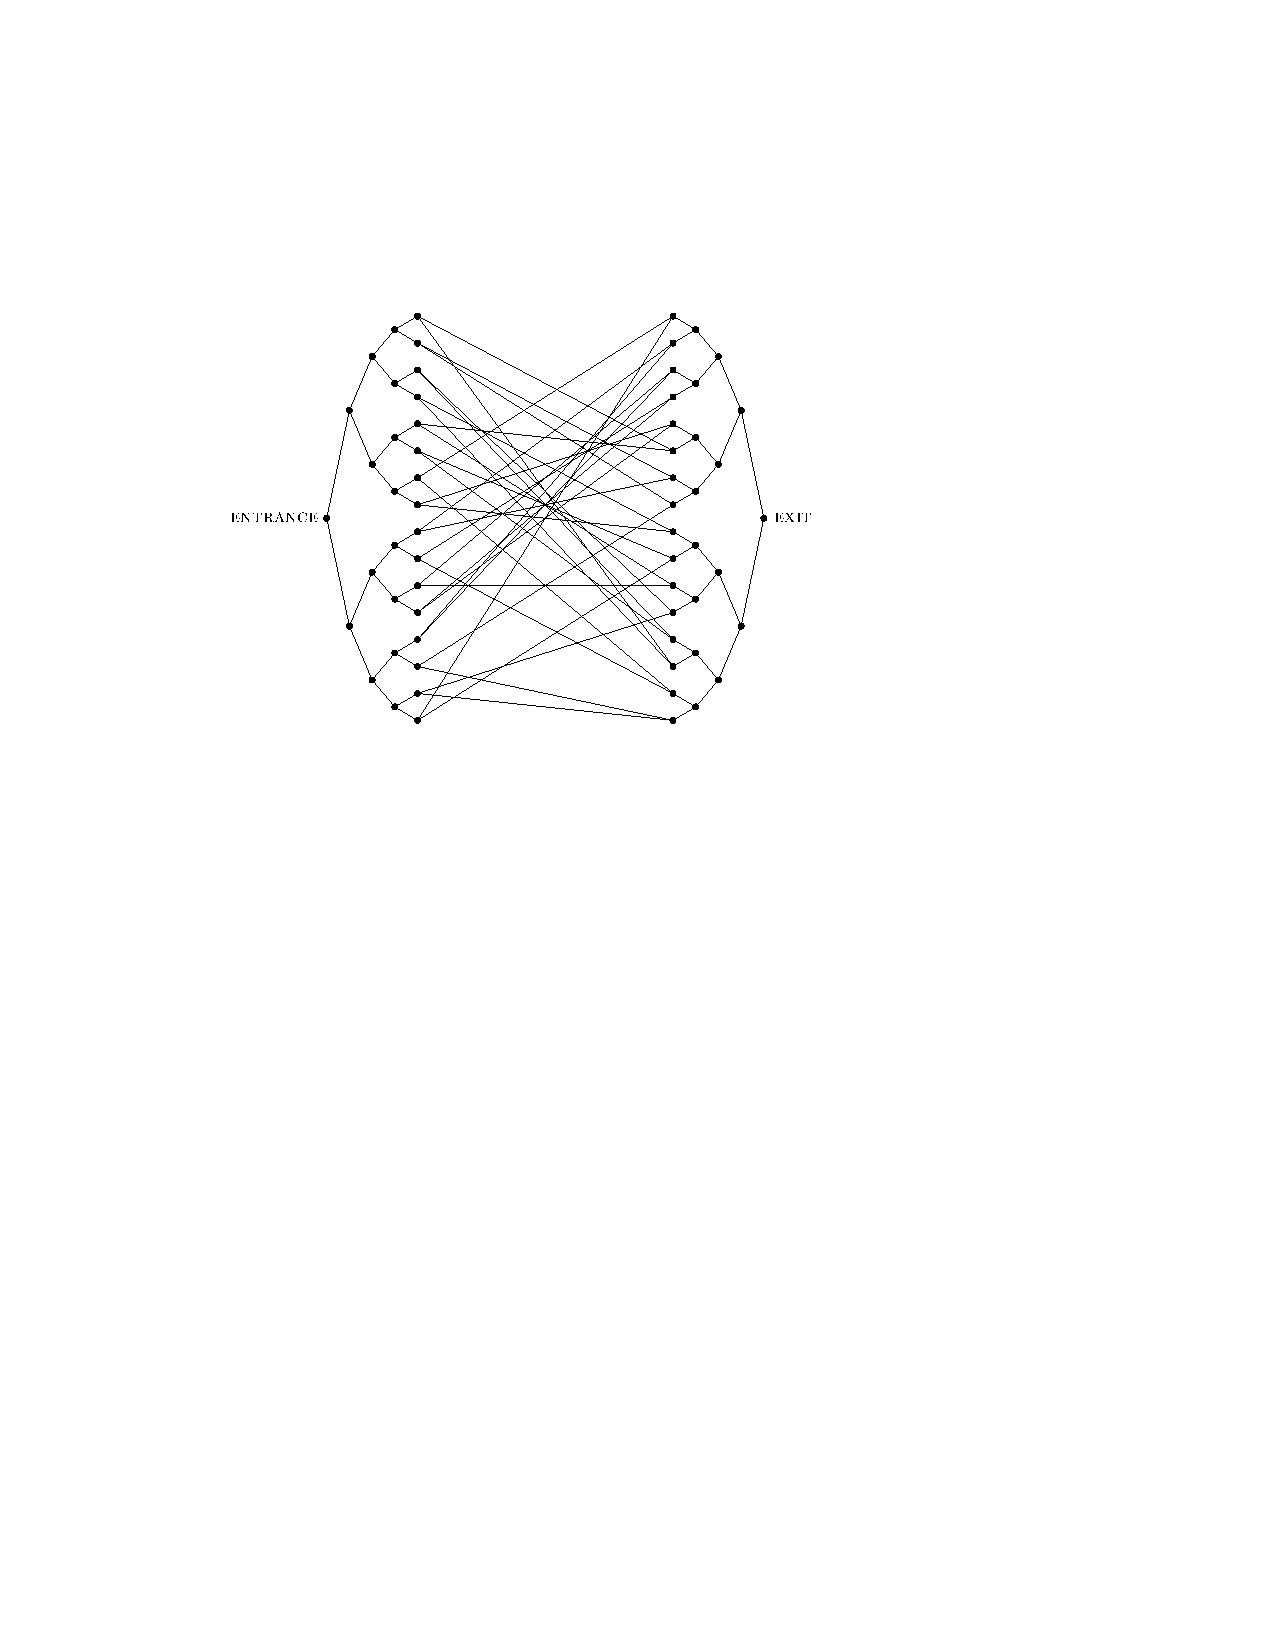
\includegraphics[width=.5\linewidth]{glued_tree.pdf}
	\caption{A typical graph exhibits rigorous exponential speedup over classical model in graph matrix representation. \cite{childsExponentialAlgorithmicSpeedup2003}}
	\label{fig:glued_tree}
\end{figure}
We have seen that the behavior of a quantum walk can be dramatically different from that of its classical counterpart. Next we will see an even stronger example of the power of quantum walk: a black-box problem that can be solved exponentially faster by a quantum walk than by any classical algorithm.
\begin{theorem}[\cite{childsExponentialAlgorithmicSpeedup2003}]
	There exists exponential (classiacl-quantum) separation with respect to query complexity under the adjacency matrix (graph) model. (glued tree)
\end{theorem}
% \cite{zhengSpeedingLearningQuantum2022};
% robust, provable speedup
% \cite{liuRigorousRobustQuantum2021}


\subsubsection{Dequantization and input assumption}
If we assume we can efficiently perform $l^2$-norm samples of input data, a natural analogue to quantum algorithms that assume efficient state preparation of classical data.
Since they are only polynomially slower, these algorithms suggest that the exponential speedups of their quantum counterparts are simply an artifact of state preparation assumptions.
\cite{tangQuantuminspiredClassicalAlgorithm2019}
\cite{tangQuantumPrincipalComponent2021}
% \begin{remark}
% 	However, when data is provided in the conventional way, i.e. from a classical computer, then the methods of [15] cannot be applied.
% \end{remark}
input model, quantum RAM;
quantum-inspired 
% \cite{tangQuantuminspiredClassicalAlgorithm2019}
% \cite{tangQuantumPrincipalComponent2021}.

\subsection{Heuristic quantum advantages for learning physics systems}
evaluate the performance on the standard graph datasets from both bioinformatics and computer vision.
Instead, we could exploit the structures inherent in physics systems and make use of quantum advantages.
problems of practical interest,
not guaranteed.
\cite{rebentrostQuantumSupportVector2014} \cite{lloydQuantumPrincipalComponent2014} etc need quantum state preparation assumptions, which state that given an input vector $v$, one can quickly form a corresponding quantum state $\ket{v}$. 

\subsubsection{Classical machine learning for quantum physics problem}
(classical) machine learning (neural network) for quantum many-body physics:
determining the phase (transition) 
a standard feed-forward neural network can be trained to detect multiple types of order parameter directly from raw state configurations sampled with Monte Carlo.
what if one was presented with a data set of Ising configurations from an unknown Hamiltonian, where the lattice structure (and therefore its T c) is not known?
We turn to the application of such techniques to problems of greater interest in modern condensed matter, such as disordered or topological phases, where no conventional order parameter exists.
Ising lattice gauge theory, one of the most prototypical examples of a topological phase of matter.
A straightforward implementation of supervised training fails to classify a test set containing samples of the two states to an accuracy over 50\% – equivalent to simply guessing. Such failures typically occur because the neural network overfits to the training set. To overcome this difficulty we consider a convolutional neural network (CNN) [4, 22] which readily takes advantage of the two-dimensional structure of the input configurations, as well as the translational invariance of the model.
\cite{carrasquillaMachineLearningPhases2017}
\cite{carleoSolvingQuantumManyBody2017}


\subsubsection{Groups and symmetries in physics and machine learning}
\cite{kondorGroupTheoreticalMethods2008};
symmetries in physics
\cite{bogatskiyLorentzGroupEquivariant2020}
\cite{bogatskiySymmetryGroupEquivariant2022};
\cite{zhengSpeedingLearningQuantum2022}?;

% \subsubsection{Group theory and machine learning}
% \cite{kondorDiffusionKernelsGraphs2002}
One of the key properties of classical CNNs is equivariance, which roughly states that if the input to the neural network is shifted, then its activations translate accordingly. 
\begin{definition}[Equivariance]\label{def:equivariant}
	Given a group $\group$ and the actions $\rho: \group \times X\to X$ and $\rho': \group \times Y\to Y$,
	a map $f: X\to Y$ is said to be \emph{equivariant} if
	\begin{equation}
		\forall x\in X, g\in \group,
		f(\rho(g,x)) = \rho'(g,f(x))
		% f(\rho_g(x)) = \rho_g'(f(x))
	\end{equation}
	% here the notation is $\rho_g(x) = \rho(g,x)$.
\end{definition}
Equivariance is one of the main reasons behind the unreasonable success of CNNs.
Combining these two is the basis of so-called Permutational Quantum Computing (PQC) [30]. Therefore, a natural starting point for realizing convolutional neural networks in quantum circuits is to look for permutational equivariance.
In particular, it has been recognized that by constructing neural networks that operate on the basis of irreducible representations of the group (so-called Fourier space neural networks), and group equivariant convolution is easy to implement because it simply reduces to matrix multiplication [32].
the quantum Fourier space activation (within PQP+) enjoys a super-exponential quantum speed-up compared with the best-known result in classical FFT over the symmetric group.
% There have been several attempts to introduce theoretically sound analogs of convolutional neural networks to quantum circuits, but they have generally been somewhat heuristic.
The major difficulty is that the key ingredient of the success of CNNs - translation invariance - lacks a mathematically rigorous quantum counterpart due to the discrete spectrum of spin-based quantum circuits.
the natural form of equivariance in quantum circuits is permutation equivariance!.
equivariant CNN 
\cite{zhengSpeedingLearningQuantum2022}.


\section{Experiments}\label{sec:experiments}

\subsection{Datasets and benchmark}
preliminary experiment;
prototypical machine learning tasks

\subsubsection{Artificial data}
we generate artificial data that can be fully separated by our feature map.

\subsubsection{Real-world dataset}
conventional graph datasets
\begin{itemize}
	\item UCI \cite{kondorDiffusionKernelsGraphs2002}, 
	\item protein [ref], 
	\item The MUTAG dataset consists of graphs representing 188 chemical compounds labeled ..;
\end{itemize}
physics datasets
\begin{itemize}
	\item particle physics: JET? \cite{bogatskiyLorentzGroupEquivariant2020}; 

	\item quantum many-body physics (phase transition)
	\cite{carrasquillaMachineLearningPhases2017} 
	topology order?
	\cite{congQuantumConvolutionalNeural2019}
% \cite{dohertyIdentifyingPhasesQuantum2009} 
\end{itemize}

\section{Discussion and Conclusion}\label{sec:discussion}
% to do 
\begin{itemize}
	\item formalize quantum graph kernels (algorithm) with quantum random walk, provable speedup
	\item quantum graph kernel for the data with group structures
	\item quantum machine learning for (practical dataset) physics problem (symmetries)
	\item whether low-depth circuit for NISQ. analog computing?
\end{itemize}

\addcontentsline{toc}{section}{References}
\printbibliography
\appendix

\section{Machine Learning and Group Theory}
% \subsection{Kernel trick in machine learning}
supervised learning: classification, regression
(SVM, neural network; gradient descent);
unsupervised learning: clustering, dimension reduction;
reinforced learning not discussed in this paper.
\subsection{Machine learning}
training set, test set.
find $f\in C$ classifier, hypothesis (concept) class. (unknow probability distribution)
The algorithm consists of two main parts: a training stage and a classification stage. 
For the training stage, a set of labeled data points are provided, on which the algorithm is performed. 
For the classification stage, we take a different set of data points and run the optimized classifying circuit on them without any label input.

\subsubsection{SVM and kernel tricks}
maximize the margin
objective (cost function): \emph{empirical risk} (error rate, loss function)
\begin{equation}
	R_{emp}(\vb{\theta}) = \frac{1}{\abs{T}}
	\sum_{\vbx\in T} \probability (\tilde{y} \neq y)
\end{equation}
the dual quadratic program that (only uses access to the kernel)
we maximize 
\begin{equation}
	L_D(\alpha) = \sum_{i=1}^t \alpha_i - \frac{1}{2}\sum_{i,j=1}^t y_i y_j \alpha_i \alpha_j \kernel(\vbx_i,\vbx_j)
\end{equation}
subject to $\sum_{i=1}^t \alpha_i y_i = 0$ and $\alpha_i\ge 0$ for each $i$?.
Lagrangian multiplier method. then dual problem
% \begin{figure}[!ht]
% 	\centering
% 	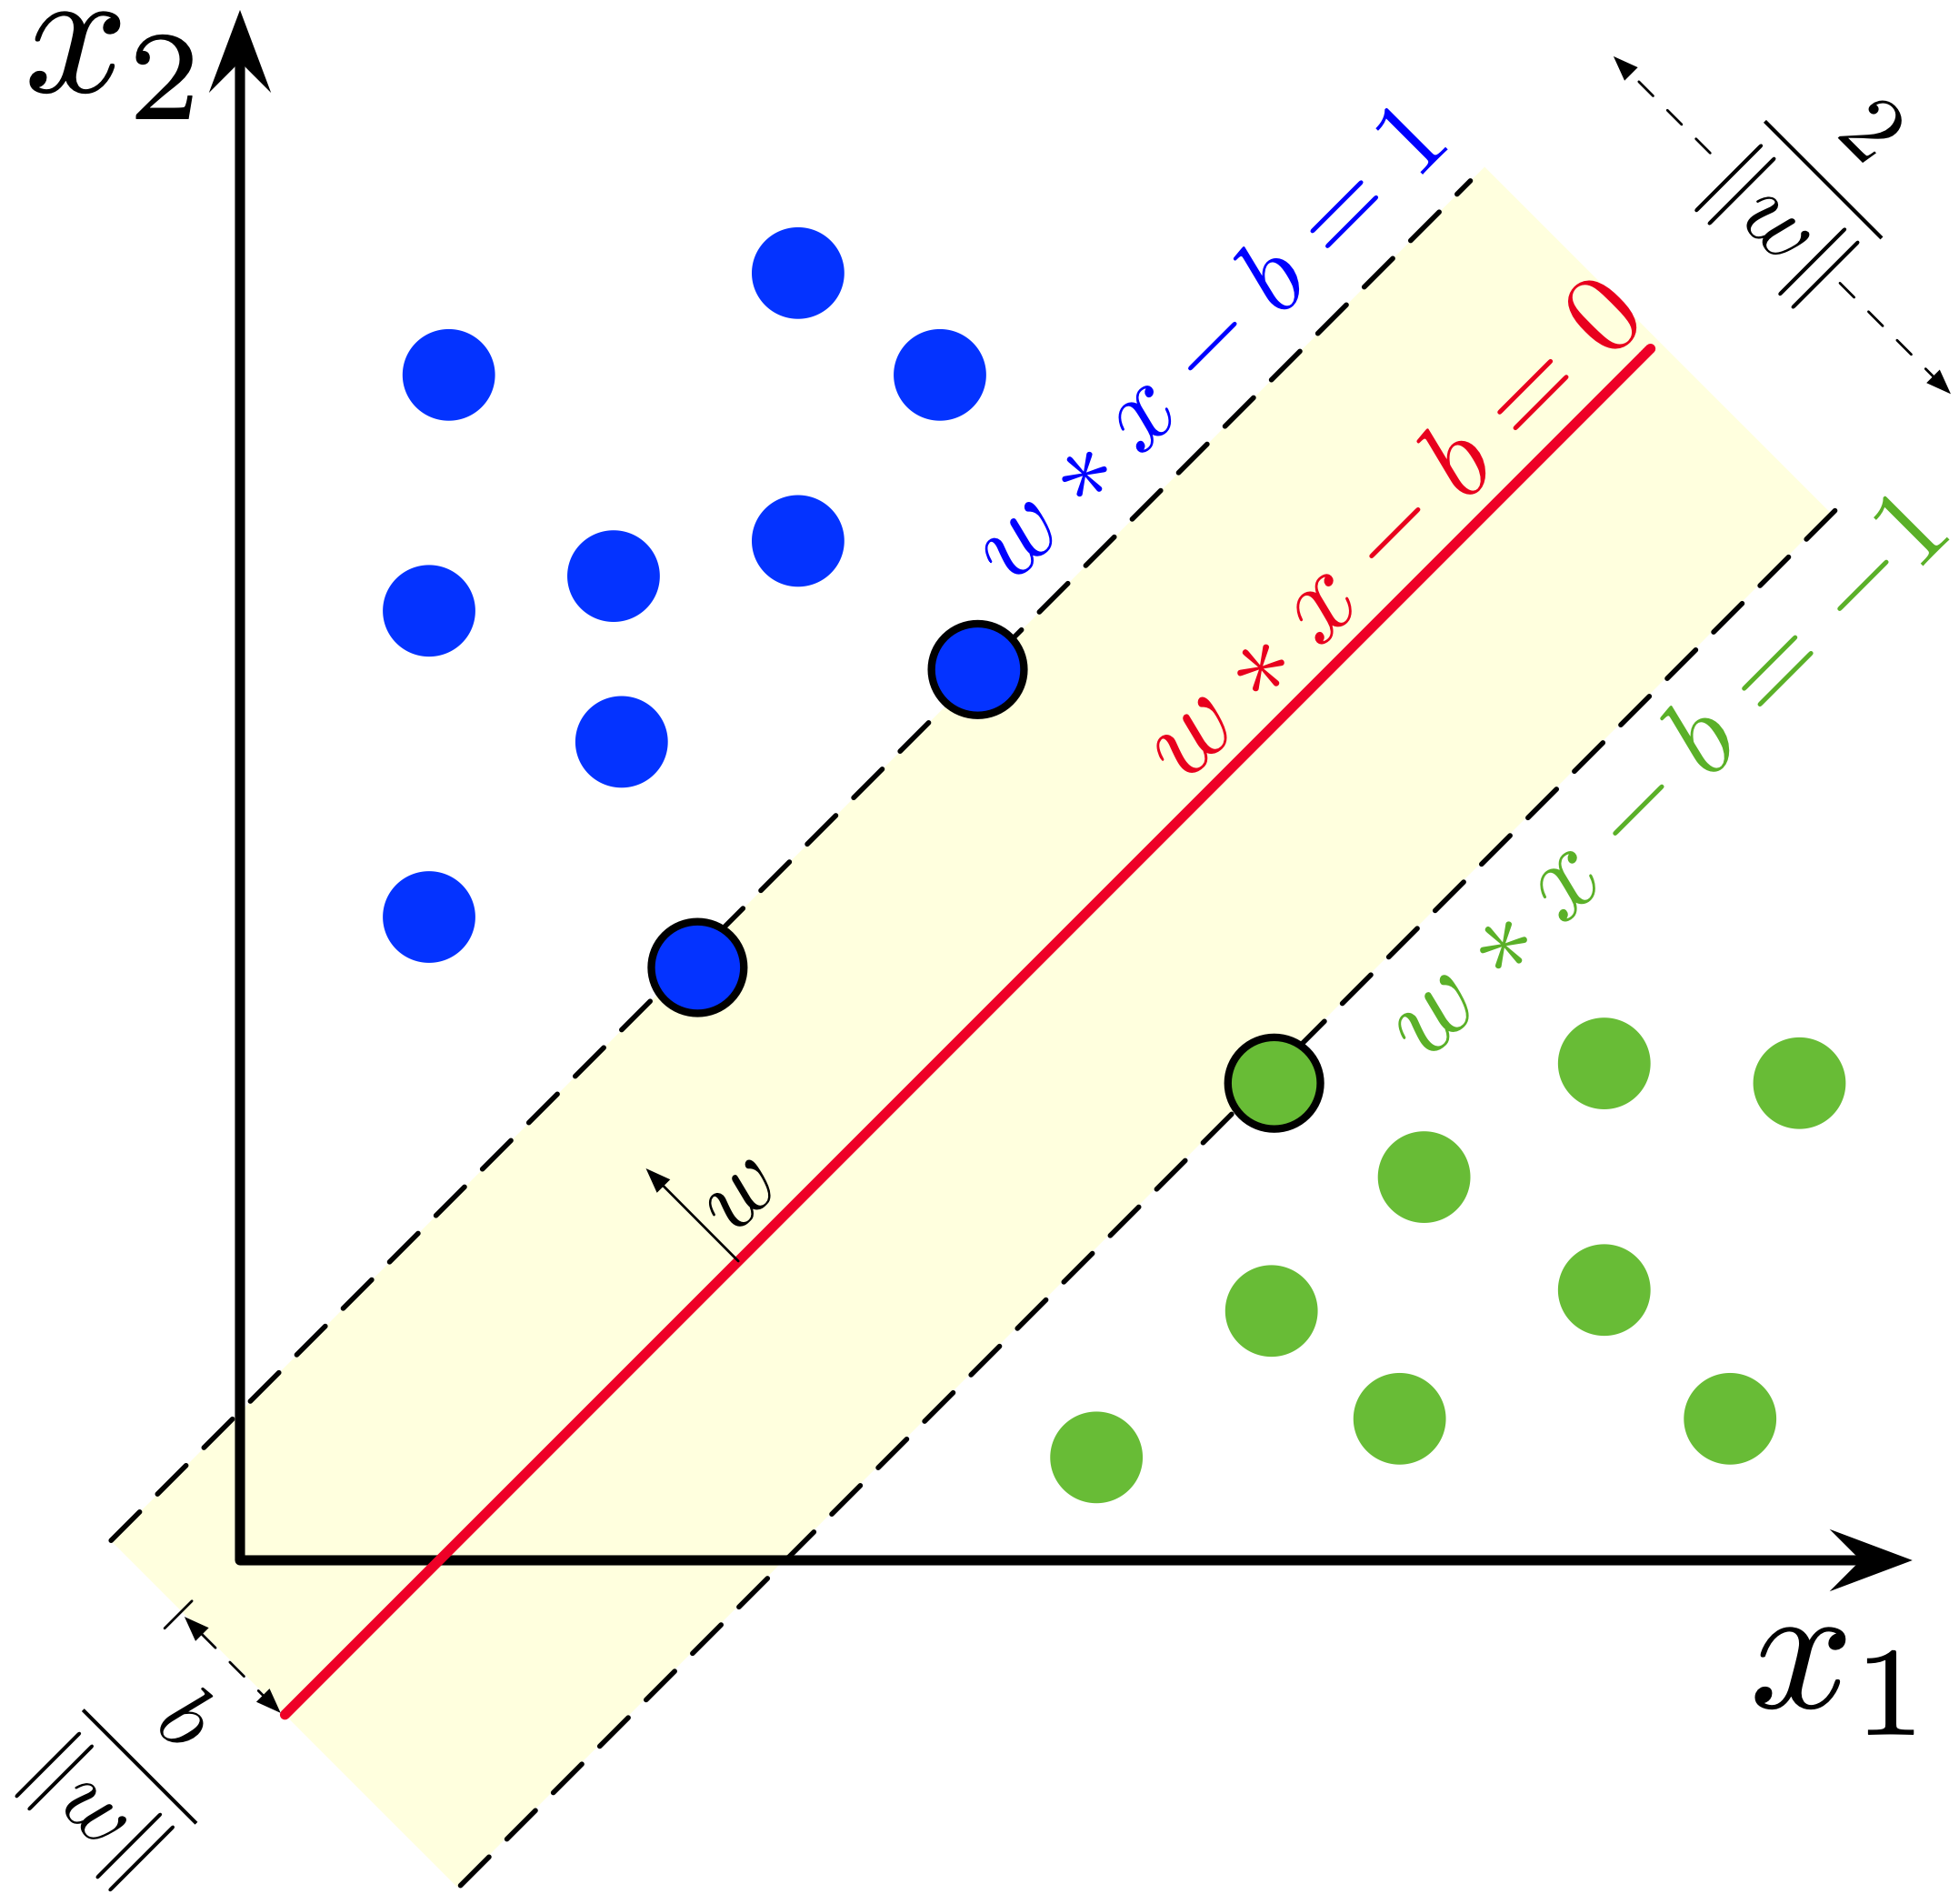
\includegraphics[width=.3\linewidth]{SVM_margin.png}
% 	\caption{linearly separable SVM}
% \end{figure}
construct the classifier
\begin{equation}
	\tilde{y}_{\textup{pred}}(\vb{s}) := \textup{sign} \qty(
		\sum_{i=1}^t y_i \alpha_i^* \kernel(\vbx_i,\vb{s}) + b
	)
\end{equation}

% \subsubsection{Neural network}

\subsubsection{Quantum machine learning}\label{sec:quantum_machine_learning}
\cite{biamonteQuantumMachineLearning2017}; 
unsupervised learning, quantum PCA \cite{lloydQuantumPrincipalComponent2014} \cite{tangQuantumPrincipalComponent2021}.
neural network,
graph neural networks (GNNs) have emerged as an alternative to graph kernels.
Quantum CNN \cite{congQuantumConvolutionalNeural2019} for quantum phase recognition and quantum error correction.
The MERA framework provides an efficient tensor network representation of many classes of interesting many-body wavefunctions, including those associated with critical systems.
The QCNN circuit has similar structure, but runs in the reverse direction.
In this sense, the QCNN circuit can mimic renormalizationgroup (RG) flow, a methodology which successfully classifies many families of quantum phases 29.

\subsection{Group theory and symmetries}
group $\group$,
permutation group $\mathbb{S}_n$;

\subsubsection{Representation theory}\label{sec:representation_theory}

\section{Symmetries in physics}
\subsection{Lagrangian formalism}\label{sec:lagrangian}
\subsubsection{Path integral and quantum computing}
\cite{xuLagrangianFormalismQuantum2021}
In optics, Fermat's principle states that the path taken by a ray between two given points is the path that can be traveled in the least (extremum) time. 
% Lagrange multiplier method
A similar argument, \emph{principle of least action}, was developed in classical mechanics:
% [\emph{Principle of least action}]
% postulate
% \begin{postulate}
% \end{postulate}
\begin{axiom}[Principle of least action]\label{thm:least_action}
    The actual path $q(t)$ taken by a classical system is the path that 
	yields an extremum of its action \(\action\).
	So, this principle is also called principle of stationary action.
	% or \emph{Hamilton's principle}.
	The action of the dynamics is the integral of Lagrangian over time
	\begin{equation}
		\action[q(t)]:=\int_{t_I}^{t_F}\dlagrangian(q(t),\dot{q}(t);t)\dd{t}
		\label{eq:action}
	\end{equation}
	where $\lagrangian(q,\dot{q})$ is the Lagrangian in terms of generalized coordinate $q$ and velocity $\dot{q}$ at certain time $t$. 
\end{axiom}
The notion $\action[\cdot]$ reminds that action is a functional that takes a function (path) $q(t)$ as input.
% see \cref{sec:path_integral} for more detail.
% (the simplest case is cartesian corrdinates, can be spherical etc)
% In classical mechanics, it is the actual path in the Euclidean space. 
By varying the action, one have the equation of motion 
% (Eq.\ref{eq:euler_lagrange}) 
called \emph{Euler-Lagrange equation}.
% \begin{equation}
%     \pdv{\lagrangian}{q_a}-\dv{t}\pdv{\lagrangian}{\dot{q}_a}=0
% \end{equation}
This Lagrangian formalism was extended by Dirac \cite{diracAnalogyClassicalQuantum1945} and Feynman \cite{feynmanQuantumMechanicsPath2010} to explain quantum mechanics. 
\begin{axiom}[Path integral]\label{thm:path_integral}
    The amplitude (probability) of a quantum system evolving from $\ket{q_I}$ to $\ket{q_F}$ in a time interval can be evaluated by (functional) integrating over all possible paths with fixed initial and final position 
    \begin{equation}
		\mel{q_F}{e^{-\ii t\hhat/\hbar}}{q_I} =
        \int_{q(t_I)= q_F}^{q(t_F)=q_I} \D q \; e^{\ii \action[q]/\hbar}
    \end{equation}
	where the action defined in classical mechanics as \cref{eq:action}.
\end{axiom}
The Larangian (path integral) formalism of quantum mechanics is proved to be equivalent to the well-known \schrodinger equation \cref{eq:evolution} \cite[Chp4]{feynmanQuantumMechanicsPath2010} 
% (complete specification)
% \begin{equation}
%     \ii\hbar \dv{t} \ket{\psi(t)} = \hhat(t) \ket{\psi(t)}
% 	% \ket{\psi}=\sum_{q} \alpha_{q} \ket{q}$, $\sum_{q} \abs{\alpha_{q}}^2=1.
%     \label{eq:evolution}
% \end{equation}
which is a differential equation determining the evolution of quantum state.
In the classical limit (Planck's constant $\hbar\to 0$), \nameref{thm:path_integral} reduces to \nameref{thm:least_action}
because only the paths around the stationary point of the action contribute 
(the other paths' contributions frequently oscillate and cancel out).
% We have included a summary of the path integral formalism for various kinds of systems in \cref{sec:path_integral}.

\subsection{Symmetries with Lagrangian}
\subsubsection{Z}
Ising model, $\integer_2$
% \begin{theorem}[Noether theorem]
% \end{theorem}

\subsubsection{U(1)}
\cite{kogutIntroductionLatticeGauge1979}
local, gauge symmetry

\subsubsection{SU(2)}
non-abelian, particle physics

\subsubsection{SO(1,3)}
Lorentz invariance
% \input{preliminary.tex}
% \input{circuit.tex}
% \input{qaoa.tex}
% \input{walk.tex}
% \input{simulation.tex}
% \input{complexity.tex}
% \input{optimization.tex}
% \input{discussion.tex}

% \section{Conclusions}

% \subsection*{Acknowledgements}
% The author thanks Yaowu Liu for his pointer to some helpful reference.
% The author thanks Andrew Childs for helpful discussion. 
% opensource software TikZiT, QuTip

%\begin{appendices}
    %\chapter{}
%\end{appendices}

% \addcontentsline{toc}{section}{References}
% \printbibliography

% \begin{widetext}
% \appendix
% \input{pathintegral.tex}
% \input{hamiltonian.tex}
% \input{cs.tex}
% \input{appendix.tex}
% \end{widetext}
% \end{appendices}
%%%%%%%%%%%%%%%Reference%%%%%%%%%%%%%%%
% \newpage

\end{document}